\documentclass[11pt,a4paper]{article}
\usepackage[margin=2.3cm]{geometry}
\usepackage{lmodern}
\usepackage[T1]{fontenc}
\usepackage[utf8]{inputenc}
\usepackage{amsmath,amssymb,amsthm}
\usepackage{booktabs,array,tabularx,longtable}
\usepackage{enumitem}
\usepackage{xcolor}
\usepackage[most]{tcolorbox}
\usepackage{titlesec}
\usepackage{graphicx}
\usepackage{tikz}
\usetikzlibrary{arrows.meta,positioning,fit,calc,shapes.geometric}
\usepackage[ruled,vlined,linesnumbered]{algorithm2e}
\usepackage[colorlinks=true,linkcolor=headblue,citecolor=headblue,urlcolor=blue!50!black]{hyperref}

\definecolor{headblue}{RGB}{38,70,120}
\definecolor{boxgray}{RGB}{245,245,242}
\titleformat{\section}{\Large\bfseries\color{headblue}}{\thesection}{0.8em}{}[{\color{black}\titlerule}]
\titleformat{\subsection}{\large\bfseries}{\thesubsection}{0.8em}{}
\titleformat{\subsubsection}{\normalsize\bfseries}{\thesubsubsection}{0.8em}{}
\setlength{\parindent}{0pt}
\setlength{\parskip}{5pt}
\setlist{itemsep=1pt,topsep=2pt}

\newtcolorbox{keybox}[1][]{colback=blue!3,colframe=headblue!60,boxrule=0.5pt,arc=2mm,left=2mm,right=2mm,top=1mm,bottom=1mm,#1}
\newtcolorbox{whybox}[1][]{colback=boxgray,colframe=black!25,boxrule=0.4pt,arc=1.5mm,left=2mm,right=2mm,top=1mm,bottom=1mm,fonttitle=\bfseries\color{black},coltitle=black,colbacktitle=boxgray,#1}

\theoremstyle{plain}
\newtheorem{proposition}{Proposition}
\theoremstyle{definition}
\newtheorem{assumption}{Assumption}[section]

% long file and folder names in \code{} may break after an underscore
\let\origunderscore\_
\renewcommand{\_}{\origunderscore\allowbreak}
\setlength{\emergencystretch}{3em}

\newcommand{\Fcs}{\mathrm{F}}
\newcommand{\Mcs}{\mathrm{M}}
\newcommand{\code}[1]{\texttt{#1}}
\newcommand{\E}{\mathbb{E}}

\hypersetup{pdftitle={Reinforcement learning for formulation 3: design and implementation of RL1 and RL2},
            pdfauthor={Yakshith Maddineni}}

\begin{document}

\begin{titlepage}
\centering
\vspace*{2.5cm}
{\LARGE\bfseries\color{headblue} Reinforcement Learning for EV Charging Assignment\\[4pt] and Mobile Charger Routing\par}
\vspace{10pt}
{\Large Design, assumptions and implementation of RL1 and RL2\par}
\vspace{18pt}
{\large CP 320 Operations Research for Mobility Management, course project\par}
\vspace{4pt}
{\large Formulation 3 (income index $\theta$)\par}
\vspace{30pt}
{\large Yakshith Maddineni (SR 26080)\par}
{\normalsize M.Tech Smart Mobility \& Logistics Systems, IISc\par}
\vspace{8pt}
{\normalsize 23 November 2026\par}
\vfill
\begin{keybox}
\textbf{What this report is.} A complete account of the reinforcement learning (RL) part of the project, written from scratch: why RL was used and why this particular RL method, which papers it is built on and what was taken from each, every assumption with its reason, the decision process in which the design was chosen, the mathematics of the environment, network, training and test-time search, the principles the code follows, the evidence collected so far, and the limits of the method.

\textbf{The two methods.} \emph{RL1} is an attention-based constructive policy (Kool et al.\ 2019) with a two-step decoder (EV, then gun or van) trained with REINFORCE and a POMO shared baseline. \emph{RL2} keeps RL1's method, changes the training where RL1 was weakest, and adds Efficient Active Search per test instance (Hottung et al.\ 2022).

\textbf{Status.} RL1 was trained and evaluated on the server: valid plans in 502 of 560 EV-Solomon instances (the 300-second MILP: 479), 1.07\,\% above the MILP plan on average, in 0.12\,s instead of 150.7\,s per instance. RL2 is implemented and tested on the laptop; its server run has not been made yet.
\end{keybox}
\end{titlepage}

\tableofcontents
\newpage

%=====================================================================
\section{Introduction}
\label{sec:intro}

\subsection{The optimisation problem in one page}

During a planning period $[0,T]$ a set $I=\{1,\dots,n\}$ of parked electric vehicles (EVs) raise charging requests. Request $i$ is released at minute $r_i$ and needs $E_i$ kWh. It must be served by exactly one resource:
\begin{itemize}
  \item a \textbf{gun} $g$ of a fixed charging station (FCS) $f(g)$ within the EV's remaining range $R_i$: the EV drives there ($d_{if}$ km, $t_{if}$ minutes), queues for at most $W_i$ minutes and charges for $\tau^\Fcs_i$ minutes; or
  \item a \textbf{mobile charging van} (MCS) $m$: the van comes from the depot or from its previous EV, the EV waits $q^\Mcs_i$ minutes and is charged for $\tau^\Mcs_i<\tau^\Fcs_i$ minutes while the driver is free.
\end{itemize}
A van serves at most $Q$ EVs, carries $B$ kWh for both driving ($\beta$ kWh/km) and delivering ($E_i/\eta$), and must be back at the depot by $T$. Every EV must be fully charged by $T$.

Every EV carries an income index $\theta_i\in[0,1]$. It sets the customer's money sensitivity $\mu_i=\mu(\theta_i)$ (non-increasing), values of time $c^{a}_i=c^{a}(\theta_i)$ for driving, queueing, charging and van service $a\in\{\mathrm D,\mathrm Q,\mathrm C,\mathrm V\}$ (non-decreasing), and queue tolerance $W_i=W(\theta_i)$ (non-increasing). The objective of formulation 3 adds the operator's cost and the cost customers perceive:
\begin{equation}
Z=\underbrace{Z_1}_{\text{EV driving}}+\underbrace{Z_2}_{\text{van km}}+\underbrace{Z_3}_{\text{dispatch}}+\underbrace{Z_4}_{\text{energy}}+\underbrace{Z_5}_{\text{tariff}}+\underbrace{Z_6}_{\text{time}} .
\label{eq:Z}
\end{equation}
The exact terms are in \code{main\_formulation\_3.pdf}, eqs.\ (1)--(23); Section~\ref{sec:mdp} restates the parts the RL environment needs. The decisions are: who serves each EV, in what order each gun and each van takes its EVs, and when each session starts.

\subsection{Why reinforcement learning at all}

The exact model is a mixed-integer linear program (MILP). The project solves it with Gurobi on 560 EV-Solomon instances (56 Solomon files, $n=10,20,\dots,100$) with a 300-second limit per instance. That run gives a reference of high quality, but it also shows the limits of exact solving:
\begin{itemize}
  \item mean solve time 150.7\,s per instance, and only 256 of 560 instances proven optimal;
  \item 30 instances end the time limit \emph{without any plan} (R1/RC1 with $n\ge70$ and one C2 instance), because the gun and queue constraints make even a first feasible solution hard to find;
  \item every new instance starts from scratch: nothing is learned from the 559 others.
\end{itemize}
A learned \emph{constructive heuristic} answers exactly these points. A neural network is trained once, offline, on many random instances drawn from the same rules as the dataset. Afterwards it builds a full plan for a new instance in a fraction of a second, it can be asked for many alternative plans in parallel, and it is not stopped by the difficulty of proving optimality. The price is that it gives no optimality guarantee: its plans are judged by comparing them with the MILP.

\subsection{What was built}

\begin{description}
  \item[RL1] (\code{RL1\_reinforcement\_learning\_method\_1/}) an attention-based policy that builds the plan one decision at a time. Each decision is a pair \emph{(EV $i$, resource $k$)}. A simulator of formulation 3 computes start times, checks feasibility, and returns the exact increase of $Z$ as the (negative) reward. Training is REINFORCE with the POMO shared baseline after a short imitation warm-up. At test time 520 plans per instance are built (8 map symmetries $\times$ 65 rollouts) and the best is kept.
  \item[RL2] (\code{RL2\_reinforcement\_learning\_method\_2/}) the same method with three changes in training (bigger batches, more large instances, a larger validation set) and \emph{Efficient Active Search}: for each test instance the trained network is frozen and the instance's embeddings are tuned on that instance for up to 10 seconds. RL1 is not changed by RL2; both read the same dataset.
\end{description}
Both write their plans in the project's common results format, and every plan is scored by the same checker (\code{check\_plan\_f3}) as the MILP and greedy plans, so the comparison is exact.

\subsection{How to read this report}

Section~\ref{sec:glossary} defines the RL vocabulary. Section~\ref{sec:chain} tells how the method was chosen, step by step, including the alternatives that were rejected. Section~\ref{sec:papers} lists the papers and what was taken from each. Section~\ref{sec:assumptions} collects every assumption with its reason and its effect. Sections~\ref{sec:mdp}--\ref{sec:inference} give the method itself: environment, network, training, and test-time search. Section~\ref{sec:principles} states the principles the implementation follows. Section~\ref{sec:evidence} gives the evidence so far, Section~\ref{sec:limits} the limits and next steps, and Section~\ref{sec:repro} how to reproduce everything.

%=====================================================================
\section{Glossary of RL terms}
\label{sec:glossary}

{\small
\begin{longtable}{@{}>{\raggedright\arraybackslash}p{3.6cm}>{\raggedright\arraybackslash}p{12.4cm}@{}}
\toprule
\textbf{Term} & \textbf{Meaning in this project} \\
\midrule
\endhead
Episode & The construction of one complete plan for one instance, from an empty plan to the moment every EV is placed (or dropped). \\
State $s_t$ & What the decision maker sees before decision $t$: which EVs are placed, when each gun becomes free, where each van is, when it is free, how much battery it has left and how many EVs it has served. \\
Action $a_t$ & One pair (EV $i$, resource $k$): EV $i$ is appended to the end of the queue of gun $k$ or to the end of the route of van $k$. \\
Mask & The set of actions that are allowed in a state. An action that would break a constraint of formulation 3 gets probability zero. \\
Reward & Minus the increase of the objective $Z$ caused by the action. Over an episode the rewards add up to $-Z$ of the plan. \\
Policy $p_\phi(a\mid s)$ & The neural network with weights $\phi$: a probability for every allowed action in the current state. \\
Rollout & One episode played by the policy, either by sampling actions from $p_\phi$ or greedily (always the most likely action). \\
Constructive heuristic & A method that builds a solution one piece at a time and never undoes a piece. The policy is a learned constructive heuristic. \\
Encoder / embedding & The part of the network that reads the whole instance once and turns every node (EV, station, depot) into a vector $h\in\mathbb R^{128}$, its \emph{embedding}, that also carries information about the other nodes. \\
Attention & The operation that lets every node weigh every other node when its embedding is computed (self-attention), and lets the decoder weigh all candidate EVs or resources when it chooses (pointer). \\
Decoder & The part of the network that is run at every step: from the embeddings and the current state it produces the action probabilities. \\
Pointer & An attention score used directly as the logit of choosing an item (Kool et al.\ 2019): the decoder ``points'' at an EV or a resource. \\
REINFORCE & The policy-gradient rule of Williams (1992): make the actions of rollouts that turned out cheaper than expected more likely, and those of dearer rollouts less likely. \\
Baseline & The ``expected'' cost that a rollout is compared with in REINFORCE. It does not change the direction of learning on average, but it reduces its noise. \\
Shared baseline & The POMO idea: roll out the same instance several times and use the mean cost of these rollouts as the baseline of each of them. \\
Advantage & How much better (negative) or worse (positive) a rollout is than its baseline; here relative: (cost $-$ baseline) / baseline. \\
Imitation / teacher forcing & Training the policy to repeat the actions of a teacher (here the greedy cost rule) by maximising their log-probability while the teacher's actions are played. \\
Map symmetry (augmentation) & One of the 8 rotations/reflections of the map around the depot. Distances do not change, so the instance is the same, but the network sees different coordinates and may build a different plan. \\
Active search & Continuing to train on one test instance only, so that the policy specialises to it (Bello et al.\ 2016). \\
Efficient Active Search (EAS) & Active search that changes only a small part of the parameters (here: the instance embeddings) while the network stays frozen (Hottung et al.\ 2022). \\
Incumbent & The best plan found so far for an instance. \\
Epoch & 50 training batches followed by one validation. \\
Validation ratio & Mean over fixed validation instances of (cost of the policy's greedy rollout) / (cost of the greedy cost rule). Below 1 means the policy beats the rule. \\
Dropped / unplaced EV & An EV for which no allowed action is left. It is counted, penalised in training, and makes the plan invalid. \\
\bottomrule
\end{longtable}}

%=====================================================================
\section{The chain of thought: how the method was chosen}
\label{sec:chain}

This section records the reasoning in the order it happened. Each step states the question that was asked, what was found, and what was decided.

\subsection{Step 1: what kind of problem is this, seen from RL?}

Before looking at any paper, five properties of formulation 3 were listed, because they decide which RL family can work at all.
\begin{enumerate}
  \item \textbf{Static, not online.} All requests of the period are known at time 0 (assumption 1 of formulation 3). The task is to write one complete plan per instance, not to react to requests as they arrive. An RL method for online dispatching would solve a different, harder problem and could not be compared fairly with the MILP.
  \item \textbf{One central decision maker.} The operator decides for every gun and every van with full information. There is no need for several learning agents that must coordinate.
  \item \textbf{Variable size.} $n$ runs from 10 to 100 (200 in the Gehring--Homberger files), and the number of resources from 24 guns + 5 vans to 48 guns + 12 vans. A method with a fixed-size input (a state vector of fixed length) would need padding or one network per size.
  \item \textbf{Hard constraints.} Queue tolerance $W_i$, deadline $T$, range $R_i$, van battery and van seats are hard. The MILP itself fails to find a feasible plan for 30 instances. Feasibility must be built into the method, not only encouraged by a penalty.
  \item \textbf{Exact evaluation exists.} \code{check\_plan\_f3} scores any plan with the formulation's own $Z$ and lists every violated constraint. Any RL method must produce a plan in the same format so that it is judged by the same rules as the MILP.
\end{enumerate}

\subsection{Step 2: what does the literature use for EV charging and routing?}

A search was made for RL in EV-charging assignment, mobile-charger routing and vehicle routing with time windows (abstracts and search results were read; the papers that were finally used were read in full). The methods fall into five families:

{\small
\begin{longtable}{@{}>{\raggedright\arraybackslash}p{3.3cm}>{\raggedright\arraybackslash}p{4.3cm}>{\raggedright\arraybackslash}p{7.7cm}@{}}
\toprule
\textbf{Family} & \textbf{Examples} & \textbf{Fit for formulation 3} \\
\midrule
\endhead
Value-based or PPO agents with a hand-made state & DQN/PPO for scheduling mobile chargers \cite{wang2023} & \textbf{Weak.} Fixed-size state and action vectors do not handle $n=10\ldots200$; they are built for online dispatch and learn a value function per state, not a complete plan. \\
Multi-agent RL & Stations or vans as agents, e.g.\ MASTER for charging recommendation \cite{master2021} & \textbf{Unneeded.} The operator decides centrally with full information (property 2). Several learners add non-stationarity and coordination problems for no gain. \\
Constructive attention policies (``learning to construct'') & Pointer networks with RL \cite{bello2016,nazari2018}, Attention Model \cite{kool2019}, POMO \cite{kwon2020}, EVRPTW \cite{lin2021}, heterogeneous fleet \cite{li2021}, Edge-DIRECT \cite{edgedirect} & \textbf{Best fit.} Size-free by construction (attention over a set of nodes), constraints enforced by masks, output is a complete plan, trained without labels. \\
Learning to improve (neural local search, neural LNS) & \cite{wu2021,hottung2020} & \textbf{Good second stage, poor first stage.} They need a feasible starting plan. Greedy fails exactly on the hard R1/RC1 instances. Repairing with a sub-MILP would mean a restricted model, which the project rules out. \\
Hybrid RL + heuristics for fixed + mobile chargers & Charging-station planning papers & \textbf{Different question.} They place stations (strategic); formulation 3 assigns and routes for one period (operational). \\
\bottomrule
\end{longtable}}

\subsection{Step 3: the choice and the reasons for it}

\begin{keybox}
\textbf{Decision.} A constructive attention policy (Attention Model family) that, at each step, chooses an EV and then a resource; trained with REINFORCE and a shared baseline (POMO); with a deterministic simulator of formulation 3 that computes all times, masks infeasible choices and returns $-\Delta Z$ as the reward.
\end{keybox}

The reasons, each tied to a property of Step 1:
\begin{enumerate}
  \item \emph{Static problem} $\Rightarrow$ a policy that writes one complete plan per episode matches the task exactly.
  \item \emph{Exact, additive objective} $\Rightarrow$ every term of $Z$ can be charged at the moment an EV is placed. The van's return leg is charged incrementally (Section~\ref{sec:reward}). So the reward is exact and adds up to $-Z$; no reward shaping is needed.
  \item \emph{Timing need not be learned.} Once the assignment and the order on each resource are fixed, starting every session as early as possible is optimal (Proposition~\ref{prop:timing}). The project's fixed-plan LP confirms it in practice: with all binaries fixed and only the times free, the LP optimum equals the plan's own cost for all 502 valid RL1 plans (whose times are earliest starts) and all 479 MILP plans. The network therefore makes only discrete choices; continuous times come from the simulator.
  \item \emph{Variable size} $\Rightarrow$ attention over a set of nodes has no fixed input size and no positional encoding; one network serves every $n$ and every number of guns and vans.
  \item \emph{Hard constraints} $\Rightarrow$ masks. Only actions that keep the plan feasible can be chosen. An EV that is left without any allowed action is dropped and the plan is flagged invalid.
  \item \emph{Two kinds of resources} $\Rightarrow$ a two-step decoder: first the EV, then its resource, as in the heterogeneous-fleet decoder of Li et al.\ \cite{li2021}. The ``fleet'' here mixes guns that stay at their station and vans that move.
  \item \emph{Simple, stable training} $\Rightarrow$ REINFORCE with a shared baseline needs no critic network (unlike PPO or actor--critic) and no second copy of the policy (unlike the greedy-rollout baseline of Kool et al.).
  \item \emph{Exact evaluation} $\Rightarrow$ the policy is just another method feeding \code{results\_io.evaluate}: its plans are scored by \code{check\_plan\_f3} exactly like MILP and greedy plans.
\end{enumerate}

\subsection{Step 4: the design questions inside the method}

Choosing the family leaves many smaller decisions. They are listed here with the alternatives that were considered.

{\small
\begin{longtable}{@{}>{\raggedright\arraybackslash}p{3.4cm}>{\raggedright\arraybackslash}p{4.4cm}>{\raggedright\arraybackslash}p{7.5cm}@{}}
\toprule
\textbf{Question} & \textbf{Options considered} & \textbf{Choice and reason} \\
\midrule
\endhead
What is one action? & (a) next node of one van (routing view); (b) resource for the next EV in release order (dispatch view); (c) pair (EV, resource) & \textbf{(c).} (a) ignores guns; (b) fixes the processing order, which loses optimal plans when a later request should take a gun first. (c) can reach every plan (Proposition~\ref{prop:complete}). \\
Who decides the times? & network outputs times; simulator & \textbf{Simulator}, earliest start (Proposition~\ref{prop:timing}). Learning a continuous time would only add noise. \\
How are constraints handled? & penalties only; masks; masks + penalty for dead ends & \textbf{Masks + a penalty} per dropped EV. Masks keep every placed EV feasible; the penalty teaches the policy to avoid leaving an EV without options. \\
What is the reward? & sparse (only $-Z$ at the end); dense $-\Delta Z$ & \textbf{Dense $-\Delta Z$}, exact. REINFORCE uses only the episode sum, but the per-step cost is also used for features (cheapest option, regret). \\
One decoder or two? & joint softmax over $n\times K$ pairs; two steps & \textbf{Two steps} (EV, then resource). The joint softmax has up to $100\times60$ outputs per step and would mix two different decisions. \\
Which baseline? & critic; greedy rollout of a frozen copy (Kool); shared mean of $S$ rollouts (POMO) & \textbf{Shared mean}, normalised by itself. No extra network, no extra rollout, scale-free across instances. \\
How to start training? & random weights; imitation of a heuristic first & \textbf{Imitation warm-up} of the greedy cost rule, then REINFORCE. On the laptop, pure REINFORCE from random weights was still 18\,\% worse than the rule after 77 batches; with the warm-up the policy matched the rule after a few hundred cheap batches. \\
Training data? & the 56 Solomon files; random instances & \textbf{Random instances} from the EV-Solomon rules (Section~\ref{sec:generator}). Within a Solomon class all files share positions, demands and $\theta$, so training on them would memorise the test set. \\
How to use test time? & one greedy rollout; sampling; sampling + augmentation; active search & RL1: \textbf{sampling + 8 map symmetries}. RL2 adds \textbf{Efficient Active Search} after the RL1 results showed that more sampling gains little (Section~\ref{sec:evidence}). \\
Symmetric resources? & offer all; offer one representative & \textbf{One representative} of identical idle guns of a station and of unused vans. Lossless and it removes probability mass spread over identical choices. \\
\bottomrule
\end{longtable}}

\subsection{Step 5: decisions forced by evidence during development}

Several choices were not made on paper but in response to what the first runs showed:
\begin{enumerate}
  \item \textbf{Imitation warm-up and the queue-position feature.} Pure REINFORCE learned slowly from random weights (validation ratio 1.18 after 77 batches). The greedy cost rule processes EVs ``stranded first, then by request time, then by income''; a network cannot copy that order unless it can see it, so a feature $f_{\text{rank}}$ (the EV's place among the open requests) was added, and the rule was taught by imitation first.
  \item \textbf{A smaller learning rate after the warm-up} (\code{lr\_reinforce} $=2\times10^{-5}$, five times smaller than the warm-up rate). At the warm-up rate the noisy policy gradient undid part of the warm-up in laptop tests.
  \item \textbf{Slower learning-rate decay on the GPU} ($0.9998$ per epoch instead of $0.998$), because the GPU runs hundreds of epochs and the old decay would have frozen learning too early.
  \item \textbf{Stopping rules} (from the user): at least 200 epochs, then early stop after 10 epochs without a better validation, at most 500 epochs; and every run starts at epoch 1, older files are archived, not deleted.
  \item \textbf{RL2.} RL1 stopped improving after about epoch 150, its gap to the MILP was largest at $n=60$--$90$, and 8$\times$ more sampling reduced the gap on seven test instances only from 1.83\,\% to 1.43\,\%. Active search on RL1's model reduced the gap on the three hardest of them from 2.76\,\% to 0.61\,\% on average. That is why RL2 combines retraining aimed at large $n$ with Efficient Active Search, and keeps RL1 untouched as the reference.
\end{enumerate}

\subsection{Step 6: rules that constrained the design}

Some project rules were fixed before the RL work began and shaped it:
\begin{itemize}
  \item \textbf{No reduced or restricted model.} The policy is offered every gun of every station and every van at every step; only infeasible pairs are masked. There are no neighbour lists or candidate shortlists.
  \item \textbf{One scorer for all methods.} RL plans go through \code{check\_plan\_f3}; the simulator is tested to give the same $Z$.
  \item \textbf{Runs never stop on one instance.} A failure becomes status \code{error} with a traceback; the run continues.
  \item \textbf{Experiments are separate.} RL2 has its own copy of the code and writes only into its own folder; RL1's code, model and results are only read.
\end{itemize}

%=====================================================================
\section{The papers and what was taken from each}
\label{sec:papers}

The implementation rests on six papers. The PDFs of the first four are in \code{RL1\_reinforcement\_learning\_method\_1/papers/}, the EAS paper in \code{RL2\_reinforcement\_learning\_method\_2/papers/}.

\begin{center}\small
\begin{tabularx}{\textwidth}{@{}>{\raggedright\arraybackslash}p{3.4cm}>{\raggedright\arraybackslash}X>{\raggedright\arraybackslash}p{2.6cm}@{}}
\toprule
\textbf{Paper} & \textbf{Taken into the implementation} & \textbf{Where in code} \\
\midrule
Kool et al.\ 2019 \cite{kool2019} & Transformer encoder over nodes without positional encoding; context + glimpse + pointer decoder; logit clipping $C\tanh(\cdot)$; masking; REINFORCE training & \code{rl2\_model.py} \\
Kwon et al.\ 2020 (POMO) \cite{kwon2020} & Shared baseline = mean cost of several rollouts of one instance; 8 map symmetries at inference & \code{train\_rl2.py}, \code{solve\_rl2.py}, \code{dihedral} in \code{rl2\_env.py} \\
Li et al.\ 2021 \cite{li2021} & Two decisions per step for a heterogeneous fleet (vehicle selection + node selection) & two-step decoder in \code{rl2\_model.py} \\
Lin et al.\ 2021 \cite{lin2021} & Evidence that masks for battery, time windows and charging work with an attention policy & masks in \code{rl2\_env.py} \\
Williams 1992 \cite{williams1992} & The REINFORCE gradient estimator & \code{train\_step} \\
Hottung et al.\ 2022 (EAS) \cite{hottung2022} & EAS-Emb: tune only instance embeddings at test time with REINFORCE + imitation of the incumbent & \code{rl2\_eas.py} (RL2 only) \\
\bottomrule
\end{tabularx}
\end{center}

\subsection{Kool, van Hoof, Welling: \emph{Attention, learn to solve routing problems!} (ICLR 2019)}

\textbf{Main idea.} A routing solution is built one node at a time by a network with two parts. The \emph{encoder} is a stack of Transformer layers (multi-head self-attention and feed-forward sublayers, Vaswani et al.\ \cite{vaswani2017}) applied to the set of nodes; because there is no positional encoding, the result does not depend on the order in which the nodes are listed, and the same weights work for any number of nodes. The \emph{decoder} is run at every construction step: it forms a context vector from the graph embedding and the current state, refines it with one multi-head attention ``glimpse'' over the nodes, and then computes single-head compatibilities with every node. These are clipped, $u=C\tanh(\cdot)$ with $C=10$, masked and passed through a softmax. Training is REINFORCE with a greedy-rollout baseline.

\textbf{What was taken.} The encoder (3 layers, $d=128$, 8 heads, feed-forward 512), the glimpse-then-pointer decoder, the clipping constant $C=10$, masking of infeasible nodes, and REINFORCE.

\textbf{What was changed and why.}
\begin{itemize}
  \item Three node types (EVs, stations, depot) with their own input layers, because they carry different features.
  \item The pointer score gets an additional learned term from \emph{dynamic} features (cheapest option, regret, time pressure, \dots), because in formulation 3 the cost of an EV depends strongly on the current queues and van positions, which static embeddings cannot know. In the AM the state enters only through the context vector.
  \item The greedy-rollout baseline was replaced by POMO's shared baseline (next paper).
\end{itemize}

\subsection{Kwon et al.: \emph{POMO} (NeurIPS 2020)}

\textbf{Main idea.} Many combinatorial problems have several optimal solutions (e.g.\ a tour can start anywhere). POMO rolls out the same instance many times from different starts and uses the \emph{mean} cost of these rollouts as the REINFORCE baseline for each of them. This baseline is low-variance and needs no critic and no frozen policy copy. At inference POMO also uses \emph{instance augmentation}: the 8 symmetries of the unit square give 8 inputs that describe the same instance; the best result over all of them is kept.

\textbf{What was taken.} The shared baseline (each training instance is rolled out $S=8$ times; the baseline is their mean) and the 8 dihedral augmentations (coordinates are taken relative to the depot, so every symmetry leaves all distances unchanged).

\textbf{What was changed and why.} POMO's ``multiple optima'' come from forcing different first nodes. In formulation 3 the first decision is a pair and the rollouts differ by sampling, not by forced starts; each training instance also gets a random symmetry, which gives the same kind of diversity. The advantage is divided by the baseline (relative cost) so that cheap and expensive instances contribute on the same scale.

\subsection{Li et al.: \emph{DRL for the heterogeneous capacitated VRP} (IEEE T-Cyb 2021)}

\textbf{Main idea.} With vehicles of different types, each step has two decisions: which vehicle moves next and which customer it serves. The paper uses a vehicle-selection decoder followed by a node-selection decoder, and multiplies their probabilities.

\textbf{What was taken.} The two-step structure and $\log p(a)=\log p(\text{first choice})+\log p(\text{second}\mid\text{first})$.

\textbf{What was changed and why.} The order is reversed: first the EV, then its resource. In formulation 3 the scarce, decisive question is ``which request is handled next'', and the resource choice for a given EV is local (it depends on that EV's distances and options). Choosing the EV first also lets the resource decoder use pair features of exactly that EV (its cost and wait on every resource). The ``fleet'' contains two very different types: guns are fixed at a station and keyed by the station's embedding; vans move and are keyed by the embedding of the node where they currently are.

\subsection{Lin, Ghaddar, Nathwani: \emph{DRL for the EVRPTW} (IEEE T-ITS 2021)}

\textbf{Main idea.} An attention-based policy for electric vehicle routing with time windows and charging stations, with masks for battery level, time windows and the possibility to reach a charging station.

\textbf{What was taken.} No component directly, but the evidence that the method copes with the same kind of hard time and energy constraints as formulation 3. The design of the van masks (enough battery to serve the EV \emph{and} return; back at the depot by $T$) follows the same reasoning as their battery and time-window masks: a mask must guarantee that the partial route can still be completed.

\subsection{Williams: \emph{Simple statistical gradient-following algorithms} (Machine Learning 1992)}

\textbf{Main idea.} For a stochastic policy, $\nabla_\phi\,\E_{\pi\sim p_\phi}[c(\pi)]=\E\big[(c(\pi)-b)\,\nabla_\phi\log p_\phi(\pi)\big]$ for any baseline $b$ that does not depend on the sampled $\pi$. The gradient can be estimated from sampled rollouts.

\textbf{What was taken.} This estimator, with the shared baseline of POMO.

\subsection{Hottung, Kwon, Tierney: \emph{Efficient active search} (ICLR 2022)}

\textbf{Main idea.} Bello et al.\ \cite{bello2016} proposed \emph{active search}: keep training the model on the one test instance to be solved. It works, but updating all weights for every instance is slow and memory-hungry. EAS updates only a small subset of parameters. In \emph{EAS-Emb} (Section~3.1 of the paper) the embeddings produced by the encoder become trainable parameters for that instance, the rest of the network is frozen, and the loss is
\[
\mathcal L_{\text{RIL}}=\mathcal L_{\text{RL}}+\lambda\,\mathcal L_{\text{IL}},
\]
where $\mathcal L_{\text{RL}}$ is REINFORCE on sampled solutions and $\mathcal L_{\text{IL}}$ is the negative log-likelihood of re-generating the best solution found so far (teacher forcing). The imitation term pulls the search towards the incumbent; the paper shows (its Section~4.5) that a moderate $\lambda$ improves results on TSP and CVRP. The paper runs 200 search iterations per instance and tunes $\lambda$ and the learning rate by Bayesian optimisation on validation instances.

\textbf{What was taken.} EAS-Emb with the RL + IL loss, the shared baseline per symmetry, Adam on the embeddings, the incumbent replay, and 200 iterations.

\textbf{What was changed and why.}
\begin{itemize}
  \item In the paper's POMO implementation only the single-head keys of the last decoder layer are updated. Here all encoder outputs (EV, station and depot embeddings) are updated, because the decoder of this project uses them in several places (context mean, glimpse keys and values, EV keys, resource keys); updating only one projection would leave the others unchanged.
  \item A wall-clock cap (10 s per instance) besides the 200 iterations, so that the total solve time of 560 instances is bounded.
  \item $\lambda=0.01$ and learning rate $0.004$ were set by hand, not tuned (a limitation, Section~\ref{sec:limits}).
  \item The incumbent is selected lexicographically (fewest dropped EVs, then lowest $Z$), and it is only replaced by a strictly better plan, so EAS can never return a worse plan than the sampling step.
\end{itemize}

%=====================================================================
\section{Assumptions}
\label{sec:assumptions}

The assumptions fall into four groups: those inherited from formulation 3, those of the simulator (environment), those of learning, and those of the test-time search. Each is stated with the reason it was made and what happens if it fails. Where an assumption is in fact a provable property, the proof is in Section~\ref{sec:mdp}.

\subsection{Inherited from formulation 3}

The RL method solves exactly formulation 3; it adds no simplification of the model. In particular it inherits:
\begin{enumerate}[label=F\arabic*.]
  \item All requests of the period are known at time 0 (static problem); request $i$ cannot start before $r_i$.
  \item Each EV is served by exactly one gun or one van, one EV at a time per resource, without pre-emption; charging power is constant, so $\tau^\Fcs_i$ and $\tau^\Mcs_i$ are known.
  \item The income index $\theta_i$ and therefore $\mu_i$, $c^{a}_i$, $W_i$ are known numbers per EV (the code uses straight lines in $\theta$, \code{code/f3\_params.json}; the model needs only their monotonicity).
  \item Vans are identical (same $B$, $Q$, $c^\Fcs$), start and end at one depot, and are not recharged during the period.
  \item Distances are road km $=$ detour factor $\times$ km per grid unit $\times$ straight-line distance, and travel times are proportional to distances (one speed). Hence distances and times satisfy the \textbf{triangle inequality}, which several proofs below use.
\end{enumerate}

\subsection{Environment (simulator) assumptions}

\begin{assumption}[Earliest-start timing]\label{as:timing}
Once it is fixed which resource serves each EV and in which order, every session starts as early as possible: $S_i=\max(r_i+t_{if(g)},\,a_g)$ on a gun, $S_i=\max(r_i,\,a_m+t_{\ell_m i})$ on a van, where $a$ is the time the resource becomes free and $\ell_m$ the van's last node.

\textbf{Why.} With assignment and sequences fixed, the remaining problem in the start times is a linear program whose constraints are lower bounds of the form $S_j\ge S_i+\text{const}$ or $S_j\ge\text{const}$, plus upper bounds ($q^\Fcs_i\le W_i$, $C_i\le T$, return by $T$), and whose cost is non-decreasing in every $S_i$. The componentwise smallest schedule is therefore optimal whenever any feasible schedule exists (Proposition~\ref{prop:timing}).

\textbf{If it fails.} It cannot fail under F1--F5. It would fail if waiting were rewarded (e.g.\ a cheaper tariff later in the period), which formulation 3 does not have.
\end{assumption}

\begin{assumption}[Append-only construction]\label{as:append}
An action appends an EV to the \emph{end} of a resource's current sequence; the construction never inserts in the middle and never undoes a decision.

\textbf{Why.} It makes each step cheap and keeps the timing of already placed EVs fixed, so the reward of a step is final. It loses nothing: every feasible plan of formulation 3 can be produced by some order of appends (Proposition~\ref{prop:complete}).

\textbf{If it fails.} Not a restriction of the plan space, only of the order in which the policy must find it: a plan whose sequences the policy ``begins wrongly'' cannot be repaired within the episode. Sampling many episodes and active search compensate.
\end{assumption}

\begin{assumption}[A dead EV stays dead]\label{as:dead}
If an unplaced EV has no feasible (EV, resource) pair at some step, it has none at any later step; it is dropped at once, counted, and the episode continues with the others.

\textbf{Why.} Gun free times only grow, van batteries only shrink, van seats only fill, and by the triangle inequality a van that moves on can only get further in time and energy from any EV (Proposition~\ref{prop:dead}). Dropping at once saves useless steps and gives a clean count of failures.

\textbf{If it fails.} It cannot fail under F1--F5.
\end{assumption}

\begin{assumption}[Lossless symmetry reduction]\label{as:sym}
Of several guns of one station that become free at the same minute, only the first is offered; of the unused vans, only the first.

\textbf{Why.} Such resources are interchangeable: exchanging their labels maps any plan onto an equally costly plan. Offering only one representative removes duplicate actions (which would split the probability of one decision over identical copies) without removing any plan up to relabelling. It is the RL counterpart of the MILP's symmetry constraints (gun order and van order).

\textbf{If it fails.} It would fail if vans or guns of one station differed (different battery, power or cost); the dataset has none.
\end{assumption}

\begin{assumption}[Exact incremental reward]\label{as:reward}
The cost increase of an action is computed with the same terms as \code{check\_plan\_f3}, including the van's way back to the depot, so the rewards of a complete episode add up exactly to $-Z$ (Proposition~\ref{prop:reward}). All times and costs are computed in 64-bit floating point.

\textbf{Why.} The policy must optimise the true objective, not a proxy. 64-bit arithmetic makes the simulator's feasibility decisions agree with the checker's (tolerance $10^{-4}$); in tests the simulator's $Z$ and the checker's $Z$ agree to $10^{-6}$ relative.
\end{assumption}

\begin{assumption}[Penalty for dropped EVs]\label{as:penalty}
The training and selection cost of a rollout is $\tilde c=Z+\lambda_{\text{drop}}\,\sigma\,|D|$, where $D$ is the set of dropped EVs, $\lambda_{\text{drop}}=10$ and $\sigma$ is the instance's cost scale: the mean, over EVs, of the cheapest feasible first option.

\textbf{Why.} A dropped EV breaks the hard rule ``every request served'', so it must cost much more than serving it. Measuring the penalty in units of a typical EV's cost ($\sigma$) makes it comparable across instances whose $Z$ differ by orders of magnitude (C2 vs R1, $n=10$ vs $n=100$).

\textbf{If it fails.} Too small: the policy might drop an awkward EV to save cost. Too large: the gradient is dominated by drops and learns little about cost. At test time selection is lexicographic (fewest drops first), so the value of $\lambda_{\text{drop}}$ does not affect which plan is reported.
\end{assumption}

\begin{assumption}[Completing an invalid plan for reporting]\label{as:complete}
If the best plan still has dropped EVs, each dropped EV is appended to the resource that finishes it earliest, ignoring the limit it violates; the plan is then scored by the checker, which lists the violations, and reported with status \code{invalid\_plan}.

\textbf{Why.} The common results format needs a resource for every EV. The plan is never presented as valid: the violations are counted and the instance is reported as ``no valid plan''.
\end{assumption}

\subsection{Learning assumptions}

\begin{assumption}[Training distribution]\label{as:dist}
The policy is trained only on random instances made with the EV-Solomon rules (Section~\ref{sec:generator}) and is tested on the 56 Solomon files it has never seen. It is assumed that the test files are typical draws of these rules.

\textbf{Why.} Within a Solomon class all files share positions, demands, ranges and $\theta$; only request times differ. Training on them would mean learning the test set. Random instances from the same rules give unlimited fresh data.

\textbf{If it fails.} If the generator misses a feature of the test files (e.g.\ the exact shape of request times in one class), the policy may be worse on that class. The RL1 results by class (Table~\ref{tab:rl1class}) are the check: the mean gap to the MILP stays between 0.6\,\% and 1.6\,\% in all six classes, so no class is badly out of distribution.
\end{assumption}

\begin{assumption}[Size and fleet coverage]\label{as:size}
Training uses the templates of the 100-EV files only (12 stations, 24 guns, 5 vans) with $n\in[10,100]$; one network is used for every $n$.

\textbf{Why.} The 560 test instances are all of that size. The attention architecture is size-free, so the same weights apply to every $n$; RL2 shifts training towards large $n$, where RL1 was weakest.

\textbf{If it fails.} For the 200-EV files (24 stations, 12 vans) the network runs, but its quality there has not been measured.
\end{assumption}

\begin{assumption}[Greedy cost rule as teacher and yardstick]\label{as:teacher}
The warm-up imitates the greedy cost rule of \code{solve\_milp\_f3} (stranded EVs first, then by request time, then higher income first; each takes its cheapest feasible resource), and validation measures the policy's cost relative to that rule.

\textbf{Why.} The rule is the MILP's own warm start: cheap, deterministic, and a reasonable plan in most instances. Imitating it gives REINFORCE a sensible start. Comparing with it on fixed instances is a fast, stable measure of progress; the MILP is far too slow to be a validation yardstick during training.

\textbf{If it fails.} A teacher bias could remain. REINFORCE after the warm-up must move away from the rule to improve; RL1's validation ratio fell from 1.01 after the warm-up to 0.969, so it did.
\end{assumption}

\begin{assumption}[Hyperparameters]\label{as:hyper}
Network sizes follow Kool et al.\ (embedding 128, 8 heads, 3 layers, feed-forward 512, clipping 10). Learning rates, batch sizes, penalty and search settings were set by hand from laptop tests; none was tuned systematically.

\textbf{If it fails.} Results may be below what tuned settings would give; Section~\ref{sec:limits} lists this as a limitation.
\end{assumption}

\subsection{Test-time assumptions}

\begin{assumption}[Map symmetries]\label{as:aug}
Coordinates are taken relative to the depot and scaled; the 8 dihedral transformations (swap $x$/$y$, flip signs) leave every distance unchanged, so all 8 inputs describe the same instance and every plan is valid for all of them.

\textbf{Why.} The network is not exactly invariant to rotation, so the 8 inputs give 8 different (but equally valid) policies: a free source of diversity for sampling and for active search.
\end{assumption}

\begin{assumption}[Selection of the reported plan]\label{as:select}
Among all plans built for an instance, the reported one is the one with the fewest dropped EVs, and among those the lowest $Z$ (key $=10^{12}|D|+Z$).

\textbf{Why.} Validity first, then cost, as in the MILP comparison.
\end{assumption}

\begin{assumption}[Active search budget]\label{as:eas}
Adapting only the instance embeddings for at most 200 iterations or 10 seconds is enough to gain most of what per-instance adaptation can give; $\lambda=0.01$ and learning rate $0.004$ fit all instances.

\textbf{Why.} The EAS paper reports that embedding-only adaptation is close to full active search at a fraction of its cost, and the laptop test on RL1's model gained about 2 percentage points of gap within 30 iterations (Section~\ref{sec:evidence}). The 10\,s cap bounds the total time of 560 instances by about 1.6 hours.
\end{assumption}

\begin{assumption}[Reproducibility]\label{as:seed}
Every instance gets its own seed, computed from the run seed and a checksum of ``file\_n''. Results therefore do not depend on the order in which instances are solved, and a resumed run gives the same plans as an uninterrupted one.
\end{assumption}

%=====================================================================
\section{The environment: formulation 3 as a Markov decision process}
\label{sec:mdp}

The environment (\code{rl2\_env.py}, identical to RL1's) is a batched PyTorch simulator: it plays many episodes side by side, for many instances or many rollouts of one instance, with every quantity a tensor of shape (batch, \dots). This section defines it mathematically.

\subsection{Resources, state and initial state}

Let $G$ be the set of guns ($|G|=24$ in the 100-EV files) with station $f(g)$, and $M$ the set of vans ($|M|=5$). The resources are $K=G\cup M$. The state before decision $t$ is
\[
s_t=\Big(P_t,\;D_t,\;(a_g)_{g\in G},\;(\ell_m,a_m,b_m,\kappa_m)_{m\in M}\Big),
\]
where $P_t$ is the set of placed EVs, $D_t$ the dropped EVs, $a_g$ the minute gun $g$ becomes free, and for van $m$: $\ell_m$ its last node (0 = depot), $a_m$ the minute it is free there, $b_m$ its battery left and $\kappa_m$ the EVs it has served. Initially $P_0=D_0=\emptyset$, $a_g=0$, $\ell_m=0$, $a_m=0$, $b_m=B$, $\kappa_m=0$.

\subsection{Actions, timing and masks}

An action is a pair $(i,k)$ with $i\notin P_t\cup D_t$ and $k\in K$. Its start time, wait and finish follow Assumption~\ref{as:timing}:
\begin{align*}
\text{gun } g:&\quad S_i=\max\!\big(r_i+t_{if(g)},\,a_g\big),\quad q^\Fcs_i=S_i-r_i-t_{if(g)},\quad C_i=S_i+\tau^\Fcs_i;\\
\text{van } m:&\quad S_i=\max\!\big(r_i,\,a_m+t_{\ell_m i}\big),\quad q^\Mcs_i=S_i-r_i,\quad C_i=S_i+\tau^\Mcs_i .
\end{align*}
The pair is \textbf{feasible} (unmasked) if
\begin{align*}
\text{gun } g:&\quad d_{if(g)}\le R_i,\qquad q^\Fcs_i\le W_i,\qquad C_i\le T,\qquad \nexists\,g'<g:\ f(g')=f(g),\ a_{g'}=a_g;\\
\text{van } m:&\quad \kappa_m<Q,\qquad b_m\ \ge\ \frac{E_i}{\eta}+\beta\big(d_{\ell_m i}+d_{i0}\big),\qquad C_i+t_{i0}\le T,\\
&\quad \kappa_m>0\ \text{ or } m \text{ is the first van with } \kappa=0 .
\end{align*}
Each condition is one constraint of formulation 3 checked at the moment of placing: reachable station (the set $G_i$), queue tolerance (eq.\ 5), deadline (eq.\ 21), seats (eq.\ 15), battery with the way home (eq.\ 16), van back by $T$ (eq.\ 19); the last condition of each block is the symmetry reduction (Assumption~\ref{as:sym}). The van battery condition reserves the energy to drive home from $i$; because of the triangle inequality, later EVs on the route can only add to that reserve, never invalidate it.

An EV is \textbf{selectable} if it has at least one feasible pair. Before every decision, EVs that are not placed and have no feasible pair are moved to $D_t$ (Proposition~\ref{prop:dead} shows they could never be placed later). The episode ends when $P_t\cup D_t=I$.

\subsection{Transition}

After action $(i,k)$: $P_{t+1}=P_t\cup\{i\}$, and
\begin{align*}
\text{gun } g:&\quad a_g\leftarrow C_i;\\
\text{van } m:&\quad b_m\leftarrow b_m-\frac{E_i}{\eta}-\beta\,d_{\ell_m i},\quad \ell_m\leftarrow i,\quad a_m\leftarrow C_i,\quad \kappa_m\leftarrow\kappa_m+1 .
\end{align*}
The simulator is deterministic: the same action sequence always gives the same plan. RL2's active search relies on this to replay the incumbent (Section~\ref{sec:eas}).

\subsection{Reward}
\label{sec:reward}

The reward is $-\Delta Z$ with
\begin{align*}
\Delta Z(i,g)=&\ \mu_i\big(c^{\mathrm{EV}}d_{if(g)}+p^\Fcs E_i\big)+\pi^\Fcs E_i+c^{\mathrm D}_i t_{if(g)}+c^{\mathrm Q}_i q^\Fcs_i+c^{\mathrm C}_i\tau^\Fcs_i,\\
\Delta Z(i,m)=&\ \mu_i\,p^\Mcs E_i+\pi^\Mcs\frac{E_i}{\eta}+c^{\mathrm V}_i\big(q^\Mcs_i+\tau^\Mcs_i\big)+c^\Mcs\big(d_{\ell_m i}+d_{i0}-d_{\ell_m 0}\big)+c^\Fcs\,[\kappa_m=0].
\end{align*}
The van term charges the detour: the van used to end its route by driving $\ell_m\to0$; now it drives $\ell_m\to i\to0$.

\begin{proposition}[The rewards add up to the objective]\label{prop:reward}
If an episode places every EV, the sum of its $\Delta Z$ equals $Z$ of eq.~\eqref{eq:Z} for the resulting plan.
\end{proposition}
\begin{proof}
$Z_1$, $Z_4$, $Z_5$ and $Z_6$ are sums of per-EV terms, and each EV's terms appear in $\Delta Z$ exactly once, when it is placed. $Z_3$: the dispatch cost $c^\Fcs$ is charged when a van serves its first EV ($\kappa_m=0$), so once per used van. $Z_2$: for a van with route $0\to i_1\to\cdots\to i_k\to0$ the van terms are
\[
c^\Mcs\big[(d_{0i_1}+d_{i_10}-d_{00})+(d_{i_1i_2}+d_{i_20}-d_{i_10})+\dots+(d_{i_{k-1}i_k}+d_{i_k0}-d_{i_{k-1}0})\big],
\]
which telescopes (with $d_{00}=0$) to $c^\Mcs\big(d_{0i_1}+d_{i_1i_2}+\dots+d_{i_{k-1}i_k}+d_{i_k0}\big)$, the length of the route.
\end{proof}

\subsection{Three properties that justify the design}

\begin{proposition}[Earliest start is optimal]\label{prop:timing}
Fix the resource of every EV and the order of the EVs on every gun and van. If some start times $S$ satisfy all constraints of formulation 3, then the earliest-start times $S^{*}$ of the simulator satisfy them too, and $Z(S^{*})\le Z(S)$.
\end{proposition}
\begin{proof}
With assignment and sequences fixed, the constraints on $S$ are (a) lower bounds: $S_i\ge r_i+t_{if}$ (FCS) or $S_i\ge r_i$ and $S_i\ge t_{0i}$ for the first EV of a van; $S_j\ge S_i+\tau^\Fcs_i$ for consecutive EVs on a gun; $S_j\ge S_i+\tau^\Mcs_i+t_{ij}$ for consecutive EVs of a van; and (b) upper bounds: $S_i-r_i-t_{if}\le W_i$, $S_i+\tau_i\le T$, $S_i+\tau^\Mcs_i+t_{i0}\le T$ for the last EV of a van. $S^{*}$ sets every $S_i$ to the largest of its lower bounds, going along each sequence. By induction along the sequences, any $S$ satisfying (a) has $S\ge S^{*}$ componentwise. Every upper bound in (b) has the form $S_i\le\text{const}$, so if $S$ satisfies it, so does $S^{*}\le S$. Finally, $S$ enters $Z$ only through $c^{\mathrm Q}_iq^\Fcs_i$ and $c^{\mathrm V}_iq^\Mcs_i$ with $q=S_i-\text{const}$ and non-negative coefficients, so $Z$ is non-decreasing in every $S_i$ and $Z(S^{*})\le Z(S)$.
\end{proof}

\begin{proposition}[No plan is out of reach]\label{prop:complete}
For every feasible plan $\pi$ of formulation 3 there is a sequence of unmasked actions whose resulting plan has the same assignment and sequences as $\pi$ (up to exchanging identical guns of one station or identical vans) and a cost no larger than $Z(\pi)$.
\end{proposition}
\begin{proof}
Order the EVs by their start time in $\pi$ (ties by position in their sequence) and append them in that order to their resource in $\pi$. Each resource's sequence is then rebuilt in its own order, and when EV $i$ is appended its predecessor is the last EV of that resource. By induction, the simulator's start times are not later than $\pi$'s (Proposition~\ref{prop:timing} applied to the prefix), so the queue, deadline and return conditions hold. The van seat count never exceeds $\pi$'s. For the battery: in $\pi$ the energy of the whole route fits in $B$; the energy still needed after reaching $i$ is $E_i/\eta$ plus the energy of the rest of the route, and by the triangle inequality the rest of the route home is at least $d_{i0}$ long, so the mask condition $b_m\ge E_i/\eta+\beta(d_{\ell_m i}+d_{i0})$ holds. If the symmetry rule hides the gun or van used in $\pi$, an identical one is offered; exchanging the two labels for the rest of $\pi$ changes nothing. The cost is at most $Z(\pi)$ by Proposition~\ref{prop:timing}.
\end{proof}

Proposition~\ref{prop:complete} is why the action space is a \emph{pair} (EV, resource): the optimal plan is always reachable. Had the EVs been processed in a fixed order (e.g.\ by request time) and only the resource been chosen, plans in which a later request is served before an earlier one on the same resource would be out of reach.

\begin{proposition}[A dead EV stays dead]\label{prop:dead}
If an unplaced EV $i$ has no feasible pair in state $s_t$, it has none in any later state.
\end{proposition}
\begin{proof}
Guns: $a_g$ never decreases, so $S_i$, $q^\Fcs_i$ and $C_i$ never decrease and the range condition never changes; a gun hidden by the symmetry rule has the same $a_g$ as the offered one. Used vans: after van $m$ serves some $j$, $\kappa_m$ grows; its start for $i$ is $\max(r_i,C_j+t_{ji})\ge\max(r_i,a_m+t_{\ell_m j}+t_{ji})\ge\max(r_i,a_m+t_{\ell_m i})$ by the triangle inequality, so it is not earlier; and the battery shortfall $E_i/\eta+\beta(d_{ji}+d_{i0})-b'_m$ with $b'_m=b_m-E_j/\eta-\beta d_{\ell_m j}$ exceeds the old shortfall by $E_j/\eta+\beta(d_{\ell_m j}+d_{ji}-d_{\ell_m i})>0$. Unused vans are identical and unchanged. So every condition that failed still fails.
\end{proof}

\subsection{One step of the simulator}

\begin{algorithm}[H]
\caption{One construction step (all rows of the batch at once)}
\DontPrintSemicolon
compute for every unplaced EV $i$ and resource $k$: $S_i$, $q_i$, $C_i$, feasibility, $\Delta Z(i,k)$ \tcp*{\code{Env.options}}
move EVs with no feasible pair to $D$ \tcp*{\code{Env.drop\_dead}}
\If{all EVs are placed or dropped}{\Return}
policy chooses EV $i$ among selectable EVs, then resource $k$ among feasible resources of $i$\;
cost $\leftarrow$ cost $+\Delta Z(i,k)$; record resource, $S_i$, $C_i$, step number of $i$\;
update $a_g$ (gun) or $(\ell_m,a_m,b_m,\kappa_m)$ (van) \tcp*{\code{Env.step}}
\end{algorithm}

\subsection{From an episode to a plan}

\code{plan\_of} turns one finished episode into the plan format of the project: the resource of every EV (``FCS$f$-gun$g$'' or ``van$v$'', vans in use numbered $1,2,\dots$ as in the MILP), start and completion times, and each van's route $0\to\dots\to0$. Dropped EVs are completed as in Assumption~\ref{as:complete}. The plan then goes through \code{results\_io.evaluate}, which calls \code{check\_plan\_f3} and writes \code{runs.csv} and \code{plan.csv}. The simulator's $Z$ is compared with the checker's and a warning is written if they differ by more than $10^{-6}$ relative.

%=====================================================================
\section{The policy network}
\label{sec:network}

The network (\code{rl2\_model.Policy}, the same architecture in RL1 and RL2) has 765\,474 parameters. Figure~\ref{fig:arch} shows its structure.

\begin{figure}[h]
\centering
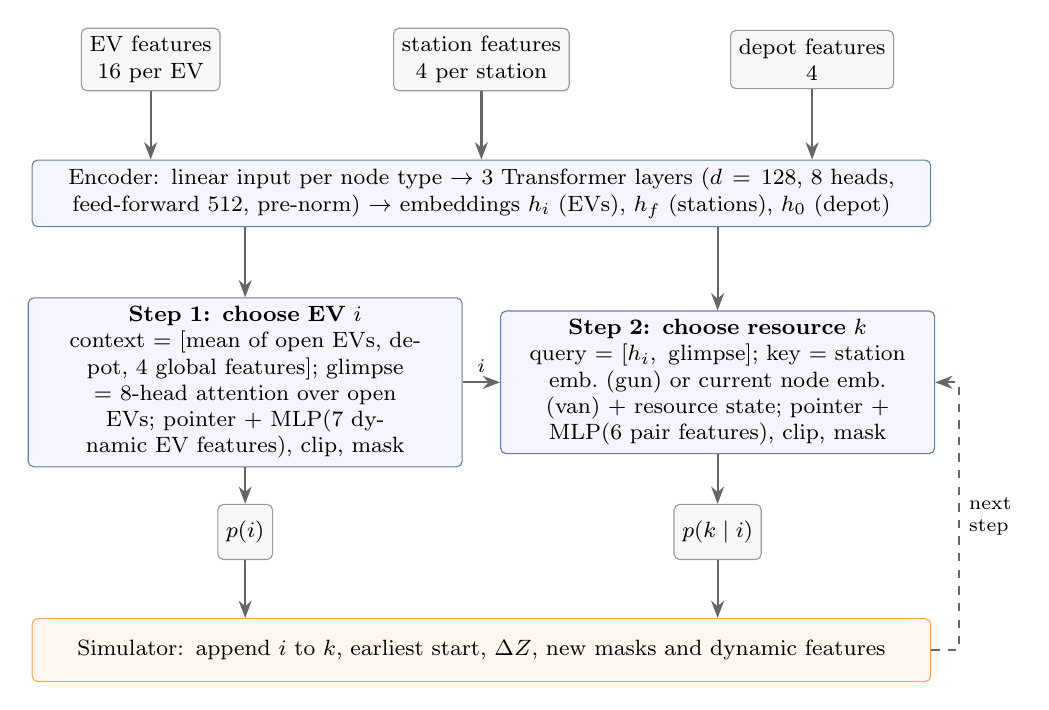
\begin{tikzpicture}[
  font=\footnotesize,
  box/.style={draw=headblue!70,fill=blue!4,rounded corners=2pt,align=center,minimum height=8mm,inner sep=3pt},
  data/.style={draw=black!40,fill=black!3,rounded corners=2pt,align=center,minimum height=7mm,inner sep=3pt},
  arr/.style={-{Stealth[length=2.2mm]},thick,draw=black!60}]
\node[data] (st) at (0,0) {station features\\ 4 per station};
\node[data] (ev) at (-4.2,0) {EV features\\ 16 per EV};
\node[data] (dep) at (4.2,0) {depot features\\ 4};
\node[box,text width=11.2cm] (enc) at (0,-1.7) {Encoder: linear input per node type $\rightarrow$ 3 Transformer layers ($d=128$, 8 heads, feed-forward 512, pre-norm) $\rightarrow$ embeddings $h_i$ (EVs), $h_f$ (stations), $h_0$ (depot)};
\draw[arr] (ev) -- (ev |- enc.north);
\draw[arr] (st) -- (enc);
\draw[arr] (dep) -- (dep |- enc.north);
\node[box,text width=5.3cm] (d1) at (-3.0,-4.1) {\textbf{Step 1: choose EV $i$}\\ context = [mean of open EVs, depot, 4 global features]; glimpse = 8-head attention over open EVs; pointer + MLP(7 dynamic EV features), clip, mask};
\node[box,text width=5.3cm] (d2) at (3.0,-4.1) {\textbf{Step 2: choose resource $k$}\\ query = $[h_i,\ \text{glimpse}]$; key = station emb.\ (gun) or current node emb.\ (van) + resource state; pointer + MLP(6 pair features), clip, mask};
\draw[arr] (enc.south -| d1) -- (d1.north);
\draw[arr] (enc.south -| d2) -- (d2.north);
\draw[arr] (d1.east) -- node[above,font=\scriptsize]{$i$} (d2.west);
\node[data] (p1) at (-3.0,-6.0) {$p(i)$};
\node[data] (p2) at (3.0,-6.0) {$p(k\mid i)$};
\draw[arr] (d1) -- (p1);
\draw[arr] (d2) -- (p2);
\node[box,text width=11.2cm,fill=orange!6,draw=orange!70] (env) at (0,-7.5) {Simulator: append $i$ to $k$, earliest start, $\Delta Z$, new masks and dynamic features};
\draw[arr] (p1) -- (p1 |- env.north);
\draw[arr] (p2) -- (p2 |- env.north);
\draw[arr,dashed] (env.east) -- ++(0.35,0) |- node[pos=0.25,right,font=\scriptsize,align=left]{next\\ step} (d2.east);
\end{tikzpicture}
\caption{Policy network and its loop with the simulator. The encoder runs once per instance (per map symmetry); the two decoder steps and the simulator run once per placed EV.}
\label{fig:arch}
\end{figure}

\subsection{Encoder}

Three node types get their own linear input layers into $\mathbb R^{128}$:
\begin{itemize}
  \item \textbf{EV} (16 static features): position relative to the depot ($x,y$, scaled, one of 8 symmetries), request time $r_i/T$, charging times $\tau^\Fcs_i/T$ and $\tau^\Mcs_i/T$, queue tolerance $W_i/T$, income $\theta_i$, energy $E_i/B$, ``stranded'' flag (no reachable station), share of reachable stations, time to the nearest reachable station, time back to the depot, range relative to the city size, cheapest gun cost and van cost (both divided by the instance's cost scale $\sigma$), and the slack $(T-r_i-\tau^\Mcs_i-t_{i0})/T$ (how late a van may come).
  \item \textbf{Station} (4): position, number of guns, share of EVs that can reach it.
  \item \textbf{Depot} (4): van seats per EV ($QM/n$), guns per EV ($|G|/n$), $\log T$, and $n/100$.
\end{itemize}
The node embeddings pass through three Transformer encoder layers (multi-head self-attention with 8 heads, feed-forward width 512, layer norm before each sublayer, no dropout) and a final layer norm. There is no positional encoding: permuting the EVs permutes the embeddings and nothing else. The encoder therefore works for any $n$, any number of stations and any number of vans.

All features are ratios or are scaled by $T$, $B$, the city size or $\sigma$, so that instances of very different size and cost (C2 with $T=3390$ minutes, R1 with $T=230$) look alike to the network.

\subsection{Decoder step 1: choose the EV}

The context vector combines the mean embedding of the EVs still open, the depot embedding and 4 global state features (share of EVs placed, mean gun busy time, share of vans in use, mean van battery left):
\[
q=W_{\text{ctx}}\,[\bar h_{\text{open}};\,h_0;\,\text{global}] .
\]
A multi-head attention ``glimpse'' over the open EVs turns $q$ into $g$. The score of EV $i$ is
\[
u_i=C\tanh\!\Big(\frac{g^\top W_K h_i}{\sqrt d}+\mathrm{MLP}(\varphi_i)\Big),\qquad C=10,
\]
masked to $-\infty$ for EVs that are not selectable, and $p(i)=\mathrm{softmax}(u)_i$. The dynamic EV features $\varphi_i$ (7) are recomputed at every step from the simulator's options: share of resources still feasible, cheapest $\Delta Z$, regret (second cheapest minus cheapest), earliest finish, cheapest gun minus cheapest van, request time relative to the earliest open request, and the EV's place in the queue of open requests ($f_{\text{rank}}$).

\begin{whybox}[title=Why dynamic features are added to the pointer]
In routing problems such as the TSP the state is almost fully described by ``where am I and what is left''. In formulation 3 the cost of an EV depends on the current gun free times and van positions, which change after every step. The static embeddings cannot know them, so the cheapest option and the regret of each EV enter the score directly. The \emph{regret} is the classical signal of insertion heuristics: an EV whose second-best option is much worse than its best should be placed before its best option is taken by another EV.
\end{whybox}

\subsection{Decoder step 2: choose the resource}

For the chosen EV $i$ the query is $q_i=W_R[h_i;g]$. The key of a resource is its base embedding plus a linear map of its current state:
\[
\text{key}_g=W_{\text{key}}h_{f(g)}+W_{\text{gun}}\,\rho_g,\qquad \text{key}_m=W_{\text{key}}h_{\ell_m}+W_{\text{van}}\,\rho_m,
\]
where $h_{\ell_m}$ is the embedding of the van's current node (depot or last EV) and $\rho$ holds 6 resource features (free time, a van flag, battery left, seats used, in use, time back to the depot; the van-only entries are 0 for a gun). The score adds an MLP of 6 pair features of $(i,k)$: $\Delta Z(i,k)/\sigma$, its excess over the cheapest option, the wait, the finish time, the van battery left after serving $i$, and a van flag. The scores are clipped, masked to the feasible resources of $i$ and normalised: $p(k\mid i)$.

The probability of the action is $p(i,k)=p(i)\,p(k\mid i)$, and the log-probability of a whole episode is the sum over its steps:
\[
\log p_\phi(\pi\mid x)=\sum_t\big[\log p(i_t)+\log p(k_t\mid i_t)\big].
\]

\subsection{Rollouts}

The function \code{rollout} plays a batch of episodes. For each row it either samples the actions from $p$, takes the most likely ones (greedy), or plays the actions of a \emph{teacher} and returns their log-probability (teacher forcing, used by the imitation warm-up and by active search). Projections that depend only on the embeddings (glimpse keys and values, EV keys, station and node keys) are computed once per batch of rollouts, not at every step.

%=====================================================================
\section{Training}
\label{sec:training}

\subsection{Training instances}
\label{sec:generator}

\code{rl2\_generator.py} makes a new random instance for every training episode, with the rules that built the EV-Solomon dataset (\code{make\_ev\_solomon.py}). From the CSV dataset it takes one \emph{template} per (file size, Solomon class): planning period $T$, depot, city area, number of stations, guns and power, costs and fleet. For each instance it then draws new customers:
\begin{itemize}
  \item \textbf{positions}: class R uniform in the city area; class C in 5--12 Gaussian clusters listed cluster by cluster (as in Solomon, so the first $n$ EVs are concentrated); class RC half clustered, half uniform;
  \item \textbf{stations}: $k$-means of all customer positions (the dataset's rule);
  \item \textbf{energy}: Solomon demand $1\ldots50$ mapped linearly onto $[10,40]$ kWh;
  \item \textbf{range}: uniform, and 15\,\% of the EVs ``stranded'' with 20--80\,\% of the distance to their nearest station;
  \item \textbf{request times}: a share (15--30\,\%) at time 0, the rest $T\cdot u\cdot\mathrm{Beta}(a,b)$ with $u\in[0.83,0.92]$, $a=1$, $b=2.5$, rounded to minutes (fitted to the dataset's request times);
  \item \textbf{income}: $\theta\sim\mathrm{Beta}$ with the parameters of \code{f3\_params.json};
  \item \textbf{period}: the class's $T$ times a random factor in $[0.85,1.15]$.
\end{itemize}
As in the dataset, an instance is the first $n$ EVs of a full random file of 100. Each instance of a batch gets a random class and a random map symmetry.

\subsection{Phase 1: imitation warm-up}

For the first 500 batches (10 epochs) the greedy cost rule plays every episode and the policy learns to reproduce its actions:
\[
\mathcal L_{\text{IL}}(\phi)=-\frac1n\,\frac1B\sum_{b=1}^{B}\sum_{t}\log p_\phi\big(a^{\text{rule}}_{b,t}\mid s_{b,t}\big).
\]
A warm-up batch is about 8 times cheaper than a REINFORCE batch, because each instance is played once instead of $S=8$ times.

\begin{whybox}[title=Why a warm-up]
From random weights the untrained policy costs 1.4--1.8 times the greedy rule on the validation instances (RL1 server log: 1.43 at epoch 0). On the laptop, pure REINFORCE needed many batches to approach the rule (1.18 after 77 batches), while imitation reached about 1.00 after a few hundred cheap batches; on the server the first warm-up epoch already gave 1.014. REINFORCE then starts from a sensible policy and only has to learn where to deviate from the rule.
\end{whybox}

\subsection{Phase 2: REINFORCE with a shared baseline}

Each batch has $B$ random instances with the same $n$ (64 in RL2, 32 in RL1). The encoder runs once per instance; every instance is then rolled out $S=8$ times by sampling. For rollout $j$ of instance $b$ let $\tilde c_{bj}$ be its penalised cost (Assumption~\ref{as:penalty}). The baseline and the advantage are
\[
\bar c_b=\frac1S\sum_{j=1}^{S}\tilde c_{bj},\qquad A_{bj}=\frac{\tilde c_{bj}-\bar c_b}{\bar c_b},
\]
and the loss whose gradient is the REINFORCE estimator is
\[
\mathcal L_{\text{RL}}(\phi)=\frac{1}{BS}\sum_{b,j}A_{bj}\,\log p_\phi(\pi_{bj}\mid x_b),\qquad
\nabla_\phi\mathcal L_{\text{RL}}\approx\nabla_\phi\,\E\Big[\frac{\tilde c}{\bar c}\Big].
\]
Rollouts cheaper than their instance's mean get a negative advantage, and the gradient step makes their actions more likely.

\begin{whybox}[title=Why this baseline and this normalisation]
\begin{itemize}
  \item The mean of the other rollouts of the same instance is a good estimate of ``what this policy usually achieves on this instance'', without a critic network to train and without the extra greedy rollout of a frozen policy copy that Kool et al.\ use.
  \item The mean includes the rollout itself; this multiplies the expected gradient by $(S-1)/S$ but does not change its direction.
  \item Dividing by $\bar c_b$ makes the advantage a relative cost. $Z$ differs by orders of magnitude between classes and sizes; without the division, the largest instances would dominate every batch.
\end{itemize}
\end{whybox}

\textbf{Optimiser.} Adam, gradient norm clipped at 1.0. Learning rate $10^{-4}$ during the warm-up and $2\times10^{-5}$ for REINFORCE, both multiplied by $0.9998^{\text{epoch}}$.

\subsection{Validation, stopping and saving}

After every epoch (50 batches) the policy's \emph{greedy} rollout is compared with the greedy cost rule on fixed validation instances (seed 777):
\[
\text{ratio}=\text{mean over validation instances of }\ \frac{\tilde c(\text{policy, greedy})}{\tilde c(\text{greedy rule})}.
\]
The network of the epoch with the lowest ratio is saved as \code{model\_best.pt}; the solver uses this one. Training stops at the first of:
\begin{itemize}
  \item \code{max\_epochs} $=500$ epochs in total;
  \item early stop: 10 REINFORCE epochs in a row without a better ratio, counted only after the first \code{min\_epochs} $=200$ epochs (so the earliest stop is at epoch 210);
  \item the time cap (8 hours).
\end{itemize}
Every run starts at epoch 1 with new weights; the files of the previous run are moved to \code{model/previous\_runs/<date-time>/}. A batch that fails is logged and skipped (training stops only after 20 failures in a row), and Ctrl-C saves the model first.

\subsection{What RL2 changes in training, and why}

\begin{center}\small
\begin{tabular}{@{}lll@{}}
\toprule
\textbf{Setting} & \textbf{RL1} & \textbf{RL2} \\
\midrule
instances per batch & 32 & 64 \\
rollouts per batch ($B\times S$) & 256 & 512 \\
distribution of $n$ in a batch & uniform on $[10,100]$ & $P(n)\propto n$ on $[10,100]$ \\
mean training $n$ & 55.0 & 67.5 \\
share of batches with $n\ge60$ & 45\,\% & 66\,\% \\
validation instances & $3\times24=72$ ($n=20,50,100$) & $4\times50=200$ ($n=20,50,80,100$) \\
\bottomrule
\end{tabular}
\end{center}

\begin{figure}[h]
\centering
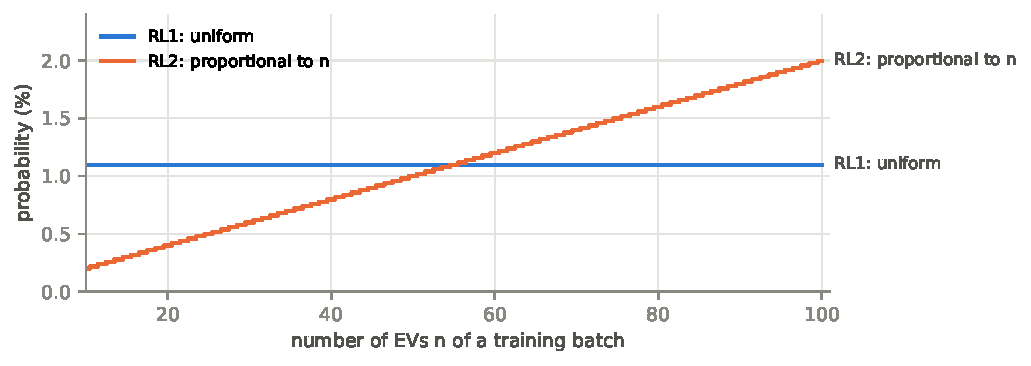
\includegraphics[width=0.85\textwidth]{figures/rl2_n_weighting.pdf}
\caption{Probability of each $n$ for a training batch. RL2 draws $n$ with probability proportional to $n$, so large instances, where RL1 lost most against the MILP, are trained more often.}
\label{fig:nweight}
\end{figure}

\begin{enumerate}
  \item \textbf{Batch 64.} The variance of the gradient estimate falls roughly as $1/(BS)$. RL1's validation ratio moved by $\pm0.003$ from epoch to epoch after epoch 150 (Figure~\ref{fig:train}), so a less noisy gradient is the first thing to try. An epoch takes about twice as long.
  \item \textbf{$P(n)\propto n$.} RL1's gap to the MILP rises from 0.5\,\% at $n=10$ to 1.5--1.7\,\% at $n=60$--$90$ (Figure~\ref{fig:gapn}). Weighting by $n$ trains these sizes more often while still covering small $n$. A batch with large $n$ also has more decisions, so more of the learning signal comes from the hard part of the plan.
  \item \textbf{200 validation instances.} The best epoch is chosen as the minimum of a noisy curve, which favours an epoch that was lucky on the validation set. With 200 instances instead of 72 the standard error of the ratio falls by a factor of about $\sqrt{200/72}\approx1.7$, and $n=80$ is now checked directly.
\end{enumerate}

%=====================================================================
\section{Solving a test instance}
\label{sec:inference}

A test instance is one CSV file of \code{dataset\_ev\_solomon/csv} and its first $n$ EVs, exactly as for the MILP. RL2 writes two runs per instance.

\subsection{Step 1: sampling with map symmetries (run \code{rl2\_sampling}, method RL2; as RL1)}

The encoder is run for the 8 map symmetries of the instance. For each symmetry the policy builds 1 greedy plan and 64 sampled plans, $8\times65=520$ plans in all. The reported plan is the one with the fewest dropped EVs, and among those the lowest $Z$ (Assumption~\ref{as:select}). Its action sequence and the 8 instance embeddings are kept for step 2.

\subsection{Step 2: Efficient Active Search (run \code{rl2\_eas}, method RL2-EAS; new in RL2)}
\label{sec:eas}

\begin{keybox}
\textbf{Idea.} The trained network is a policy for \emph{all} instances of the training distribution. Active search specialises it to the \emph{one} instance being solved, by continuing to train on that instance only. Efficient active search does this cheaply: the network is frozen and only the instance's embeddings move.
\end{keybox}

Let $\psi_a=(h^{a}_{\text{EV}},h^{a}_{\text{station}},h^{a}_{\text{depot}})$ be the encoder output for symmetry $a=1,\dots,8$; these become trainable parameters, initialised with the encoder output. All network weights $\phi$ are frozen. Let $\pi^\star$ be the incumbent (step 1's best plan) and $(i^\star_t,k^\star_t)$ its action sequence. Each iteration:
\begin{enumerate}
  \item sample $S'=32$ plans per symmetry with the current $\psi_a$ ($8\times32=256$ plans);
  \item REINFORCE loss with the shared baseline per symmetry:
  \[
  \mathcal L_{\text{RL}}(\psi)=\frac{1}{8S'}\sum_{a,j}\frac{\tilde c_{aj}-\bar c_a}{\bar c_a}\log p_\phi(\pi_{aj}\mid\psi_a);
  \]
  \item imitation loss: replay $\pi^\star$ in every symmetry (teacher forcing) and take its mean negative log-likelihood per decision,
  \[
  \mathcal L_{\text{IL}}(\psi)=-\frac{1}{8n}\sum_{a}\log p_\phi(\pi^\star\mid\psi_a);
  \]
  \item one Adam step (learning rate 0.004) on $\psi$ for $\mathcal L_{\text{RL}}+\lambda\mathcal L_{\text{IL}}$, $\lambda=0.01$;
  \item if one of the 256 sampled plans is strictly better than $\pi^\star$ (fewer dropped EVs, or as many and a lower $Z$), it becomes the new incumbent.
\end{enumerate}
The search stops after 200 iterations or 10 seconds, whichever comes first.

\begin{algorithm}[H]
\caption{Efficient Active Search for one instance (\code{rl2\_eas.active\_search})}
\DontPrintSemicolon
\KwIn{frozen policy $\phi$; embeddings $\psi^{0}_{1..8}$; incumbent $\pi^\star$ from step 1}
$\psi\leftarrow$ trainable copy of $\psi^{0}$; Adam on $\psi$\;
\While{iterations $<200$ \textbf{and} time $<10$\,s}{
  sample $32$ plans per symmetry with $\psi$; costs $\tilde c_{aj}$, log-probabilities\;
  $\mathcal L\leftarrow\mathcal L_{\text{RL}}$ (baseline = mean per symmetry)\;
  replay $\pi^\star$ with teacher forcing in each symmetry; $\mathcal L\leftarrow\mathcal L+\lambda\mathcal L_{\text{IL}}$\;
  Adam step on $\psi$\;
  \lIf{best sampled plan $\prec\pi^\star$}{$\pi^\star\leftarrow$ that plan}
}
restore the frozen flags of $\phi$; \Return $\pi^\star$, iterations, seconds\;
\end{algorithm}

\begin{proposition}[Never worse]
The plan returned by active search has no more dropped EVs than step 1's plan, and if it has as many, a $Z$ no larger.
\end{proposition}
\begin{proof}
The incumbent starts as step 1's plan and is replaced only by a plan that is strictly better in the lexicographic order (dropped EVs, $Z$).
\end{proof}

\begin{whybox}[title=Why the embeddings and not the whole network]
\begin{itemize}
  \item \textbf{Cost.} Updating all 765\,474 weights per instance (the original active search) needs the encoder in every backward pass and a separate copy of the optimiser state per instance. Updating the embeddings needs neither: the encoder is not run again.
  \item \textbf{Expressiveness.} Every decoder decision is computed from the embeddings (context, glimpse keys and values, EV keys, resource keys), so moving them can change any action probability of this instance.
  \item \textbf{Stability.} The EAS paper reports that the learning rate is much easier to choose when only a subset of parameters moves; the trained decoder keeps its general knowledge.
\end{itemize}
\end{whybox}

\begin{whybox}[title=Why the imitation term]
REINFORCE alone moves the policy towards plans that are better than the current \emph{average}, which may still be far from the best plan found. The imitation term pulls the policy towards the incumbent, so the samples concentrate around it and explore its neighbourhood: small changes to a good plan rather than new plans from scratch. Too large a $\lambda$ would only reproduce the incumbent; $\lambda=0.01$ keeps the RL term dominant.
\end{whybox}

\textbf{Why the replay is exact.} The simulator is deterministic and the incumbent's actions were all feasible when they were taken, so replaying them from an empty plan rebuilds exactly the same plan (check 6 of \code{test\_rl2.py}). Its log-probability under the current $\psi$ is therefore well defined at every step.

\subsection{Scoring and output}

Both plans are scored by \code{check\_plan\_f3} through \code{results\_io.evaluate} and appended to \code{results/runs.csv} and \code{plan.csv} after every instance. The \code{solve\_s} of \code{rl2\_eas} includes the sampling step, so it is the full time of the method. The message column records the number of rollouts, the iterations of active search, the change in $Z$, and the iteration in which the best plan was found. \code{compare\_rl2.py} then joins RL2-EAS, RL2, RL1, greedy and the MILP per instance and by class and $n$.

\textbf{Ablation.} \code{solve\_rl2.py} with the options \code{-{}-model} (path of RL1's \code{model\_best.pt}) and \code{-{}-run-id-prefix rl1model} runs both steps with RL1's trained network (read only). Comparing \code{rl1model\_eas} with RL1 isolates the effect of active search; comparing \code{rl2\_sampling} with RL1 isolates the effect of the new training.

%=====================================================================
\section{Principles implemented in the RL programs}
\label{sec:principles}

The design follows a small number of principles. They are the ``ideology'' of the implementation: when a decision was open, these settled it.

\begin{enumerate}[leftmargin=*,label=\textbf{P\arabic*.}]
  \item \textbf{Learn only what cannot be computed.} Start times, waits, feasibility and costs follow exactly from the model, so the simulator computes them (Proposition~\ref{prop:timing}). The network decides only what has no closed form: which EV next and which resource. Fewer things to learn means faster, more reliable learning.

  \item \textbf{The objective is the reward.} The reward is the exact increase of $Z$; the rewards of an episode add up to $-Z$ (Proposition~\ref{prop:reward}). There is no hand-made shaping that could teach the policy to optimise something else. The only addition is the penalty for an EV that cannot be served, which corresponds to a hard constraint of the model.

  \item \textbf{Feasible by construction, honest about failure.} Masks make it impossible to place an EV in a way that breaks a constraint. When an EV is left without options it is not hidden: it is counted, penalised in training, and the plan is reported as invalid with its violations listed by the checker.

  \item \textbf{One judge for every method.} RL plans, MILP plans and greedy plans are all scored by \code{check\_plan\_f3} and written by \code{results\_io}. The simulator is tested to agree with the checker. A comparison between methods is therefore a comparison of plans, not of two different cost calculations.

  \item \textbf{The complete model, never a restricted one.} Every gun of every station and every van is offered at every step; only infeasible pairs are removed. No neighbour lists, no candidate shortlists, no reduced station sets.

  \item \textbf{Remove redundancy, exploit free symmetry.} Identical idle guns and unused vans are offered once (lossless, Assumption~\ref{as:sym}). The 8 map symmetries, which change the input but not the instance, are used for free diversity at test time and during active search.

  \item \textbf{Size-free and scale-free representation.} Attention without positional encoding handles any $n$ and any fleet; all features are ratios scaled by $T$, $B$, the city size or the instance's cost scale; advantages are relative costs. One network serves instances whose $Z$ differ by orders of magnitude.

  \item \textbf{Start from what is known, then improve.} Training starts by imitating the greedy cost rule and then improves on it with REINFORCE; active search starts from the best sampled plan and improves around it. Neither stage throws away what the previous one achieved.

  \item \textbf{Never worse.} At test time the best of all plans is kept, and active search can only replace the incumbent by a strictly better plan. Adding RL2's search to RL1's sampling cannot make the reported plan worse.

  \item \textbf{Generalise, do not memorise.} The policy is trained only on fresh random instances; the 56 test files are never seen in training. Validation uses separate fixed random instances.

  \item \textbf{Measure against the strongest and the simplest reference.} Every RL result is reported against the 300-second MILP (and its proven optima) and against the greedy rule. A learned method is only interesting if it is close to the first and clearly better than the second.

  \item \textbf{Separate, reproducible experiments.} RL1 and RL2 are separate folders with their own code copies, models and results; RL2 only reads RL1. Seeds are fixed per instance; every training run starts at epoch 1 and archives the previous run instead of deleting it; settings are saved with every model and result.

  \item \textbf{Long runs never die on one case.} A failed training batch is logged and skipped; a failed instance becomes a row with status \code{error} and a traceback; results are appended after every instance and \code{-{}-resume} skips what is done.
\end{enumerate}

%=====================================================================
\section{Evidence so far}
\label{sec:evidence}

\subsection{Verification of the implementation}

\code{test\_rl2.py} (identical to RL1's tests plus check 6) is run before every training:
\begin{enumerate}
  \item \textbf{Data.} The CSV loader builds exactly the instance of the MILP's text loader (RL1 full test: all 228 tested instances, 56 files $\times$ $n=10/50/100$ plus 60 Gehring--Homberger files at $n=200$).
  \item \textbf{Simulator.} The greedy cost rule played inside the simulator gives the same plan cost as \code{greedy\_f3} of the MILP code, and the simulator's $Z$ equals the checker's $Z$ (RL1: 190 instances).
  \item \textbf{Random policy.} Plans of an untrained network without dropped EVs pass the checker with no violation and the same $Z$ as the simulator; plans with dropped EVs are complete and flagged.
  \item \textbf{Generator.} Random instances of every class run through simulator and checker.
  \item \textbf{Training step.} Finite loss and gradients.
  \item \textbf{Active search (RL2).} Replaying the incumbent's actions rebuilds the same plan; a few iterations never return a worse plan; the starting embeddings are left untouched; the plan passes the checker.
\end{enumerate}
All six checks passed on the laptop (22 Nov 2026, quick mode); a 2-epoch training run and the comparison script ran end to end.

\subsection{RL1 training on the server}

RL1 was trained on an RTX 4090 (torch 2.14.1, CUDA 12.6) on 22 Nov 2026. Figure~\ref{fig:train} shows the validation ratio by $n$.

\begin{figure}[h]
\centering
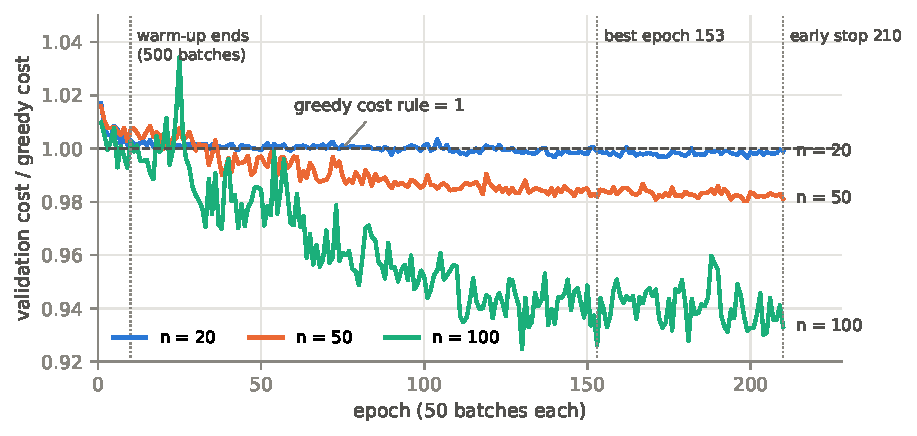
\includegraphics[width=0.9\textwidth]{figures/rl1_training_curve.pdf}
\caption{RL1 validation ratio (policy cost / greedy-rule cost, below 1 = better than the rule) per epoch, for $n=20$, $50$, $100$. Epoch 0 (untrained, 1.43 overall) is off the scale.}
\label{fig:train}
\end{figure}

\begin{itemize}
  \item Untrained: ratio 1.43. After the first warm-up epoch (50 imitation batches): 1.014.
  \item REINFORCE from epoch 11 lowered the ratio steadily to about 0.98 by epoch 75 and 0.969 at epoch 153 (best). The gain is almost entirely at large $n$: at $n=100$ the ratio fell to about 0.93, at $n=20$ it stayed near 1.00 (small instances leave little room beyond the rule).
  \item After epoch 150 the ratio moved between 0.970 and 0.975 without a new best; training stopped early at epoch 210 (10 epochs without improvement after the first 200). Total 10\,500 batches in 38.6 minutes.
\end{itemize}

\subsection{RL1 on the 560 test instances}

\begin{table}[h]
\centering\small
\caption{RL1 against the 300-second MILP and the greedy rule, by Solomon class. Gaps are $100(Z_{\text{RL1}}-Z_{\text{other}})/Z_{\text{other}}$ over instances where both plans are valid.}
\label{tab:rl1class}
\begin{tabular}{@{}lrrrrrrr@{}}
\toprule
class & inst. & \shortstack[r]{RL1\\valid} & \shortstack[r]{MILP\\valid} & \shortstack[r]{RL1 valid,\\MILP none} & \shortstack[r]{gap to\\MILP \%} & \shortstack[r]{gap to\\optimum \%} & \shortstack[r]{gap to\\greedy \%} \\
\midrule
C1 & 90 & 90 & 90 & 0 & 1.06 & 0.74 & $-1.12$ \\
C2 & 80 & 80 & 79 & 1 & 1.60 & 1.44 & $-1.04$ \\
R1 & 120 & 89 & 76 & 13 & 0.80 & 0.34 & $-1.96$ \\
R2 & 110 & 110 & 110 & 0 & 1.22 & 0.66 & $-2.57$ \\
RC1 & 80 & 53 & 44 & 9 & 1.13 & 0.75 & $-5.94$ \\
RC2 & 80 & 80 & 80 & 0 & 0.60 & 0.19 & $-4.01$ \\
\midrule
all & 560 & 502 & 479 & 23 & 1.07 & 0.74 & $-2.47$ \\
\bottomrule
\end{tabular}
\end{table}

\begin{itemize}
  \item \textbf{Feasibility.} RL1 finds a valid plan in 502 instances, the MILP in 479. In 23 instances (R1, RC1, one C2) RL1 has a valid plan where the MILP found none in 300 s; the reverse never happens. Of the 58 instances without an RL1 plan, 51 are proven infeasible (the data), so RL1 misses at most 7.
  \item \textbf{Cost.} Where both have a valid plan, RL1 is 1.07\,\% dearer than the MILP on average (median 0.89\,\%), 0.74\,\% above proven optima, and 2.47\,\% cheaper than the greedy rule (better in 366 of 474 instances).
  \item \textbf{Time.} 0.12 s per instance (520 rollouts) against 150.7 s for the MILP: about 1\,250 times faster.
  \item \textbf{Where it loses.} The gap grows with $n$ up to $n=80$ (Figure~\ref{fig:gapn}) and is largest in class C2 (long period, clustered customers).
\end{itemize}

\begin{figure}[h]
\centering
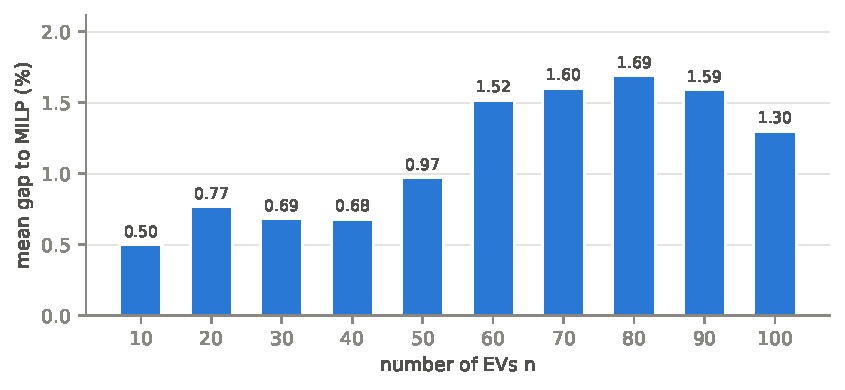
\includegraphics[width=0.85\textwidth]{figures/rl1_gap_by_n.pdf}
\caption{RL1 mean gap to the MILP plan by number of EVs (instances where both plans are valid). This profile motivated RL2's size weighting and active search.}
\label{fig:gapn}
\end{figure}

\subsection{Evidence behind RL2}

\textbf{More sampling helps little.} On seven test instances, sampling 8 times more plans per symmetry (512 instead of 64, i.e.\ 4\,104 plans instead of 520) lowered RL1's mean gap to the MILP only from 1.83\,\% to 1.43\,\%: the trained policy keeps proposing plans from the same region.

\textbf{Active search helps a lot.} Active search on RL1's trained model (the ablation of Section~\ref{sec:eas}; laptop CPU, only 30 iterations, RL1's files only read) on the three instances with the largest gaps:

\begin{center}\small
\begin{tabular}{@{}lrrrr@{}}
\toprule
instance & sampling (520 plans) & $8\times$ more sampling & active search & change in $Z$ \\
\midrule
EV-R208, $n=60$ & 3.92\,\% & 3.25\,\% & 1.25\,\% & $-2.57$\,\% \\
EV-C104, $n=90$ & 2.59\,\% & 0.97\,\% & 0.81\,\% & $-1.74$\,\% \\
EV-R112, $n=80$ & 1.76\,\% & -- & $-0.23$\,\% & $-1.96$\,\% \\
\midrule
mean gap to MILP & 2.76\,\% & & 0.61\,\% & \\
\bottomrule
\end{tabular}
\end{center}
On EV-R112 the searched plan is cheaper than the MILP's 300-second plan. The best plans were found late (iterations 23--28 of 30), so more iterations should help further; on the CPU an iteration took 6--14 s, while on the GPU it is expected to take a fraction of a second (not yet measured), so the 10-second cap should allow far more than 30.

These numbers are from three instances and must not be read as the expected average; they are the reason RL2 was built, not its result.

\subsection{What the RL2 server run will show}

\code{compare\_rl2.py} reports, per method (RL2-EAS, RL2, RL1, greedy) against the MILP: valid plans, plans where the MILP has none, mean and median gap to the MILP and to proven optima, wins against greedy, and seconds per instance, overall, by class and by $n$, plus what active search changed. Two comparisons answer the two questions of RL2:
\begin{itemize}
  \item \code{rl2\_sampling} vs \code{rl1}: did the new training (batch 64, $P(n)\propto n$, larger validation) help, especially at $n\ge60$?
  \item \code{rl2\_eas} vs \code{rl2\_sampling}: how much does active search add, and at what time cost (at most 10 s per instance)?
\end{itemize}

%=====================================================================
\section{Limitations and next steps}
\label{sec:limits}

\subsection{Limitations}

\begin{enumerate}
  \item \textbf{No optimality guarantee.} The policy is a heuristic. Its plans are judged only by comparison with the MILP; on instances the MILP cannot solve to optimality, the true gap of both is unknown.
  \item \textbf{Hard constraints can still defeat it.} Masks guarantee that every \emph{placed} EV is feasible, but a sequence of locally reasonable choices can leave a later EV without options. Such plans are reported as invalid (58 of 560 for RL1, 51 of them proven infeasible).
  \item \textbf{Training distribution.} The policy is only as good as the generator's resemblance to the test files (Assumption~\ref{as:dist}). It was trained on the templates of the 100-EV files; its quality on the 200-EV files (more stations and vans) is not measured.
  \item \textbf{Teacher bias.} The warm-up imitates the greedy rule; REINFORCE then improves on it, but some of the rule's habits may survive. The validation yardstick is also the rule, not the MILP.
  \item \textbf{Hyperparameters not tuned.} Network size follows Kool et al.; learning rates, batch sizes, penalty, and the active-search settings ($\lambda$, learning rate, samples, time cap) were set by hand. The EAS paper tunes its settings by Bayesian optimisation; this project did not.
  \item \textbf{One training run.} RL1's numbers come from one training seed. Differences between RL1 and RL2 smaller than the run-to-run variation of training cannot be attributed to the changes.
  \item \textbf{Small evidence for active search.} The active-search gain was measured on three instances on a CPU with 30 iterations. The server run on all 560 instances is the real test.
  \item \textbf{Static problem only.} Like formulation 3, the policy assumes all requests are known at time 0. It does not yet handle requests that arrive during the period.
  \item \textbf{Compute.} Training needs a GPU for a reasonable time (39 minutes on an RTX 4090 for RL1; hours on a laptop CPU). Solving is cheap on any machine.
\end{enumerate}

\subsection{Next steps}

\begin{enumerate}
  \item \textbf{Run RL2 on the server} and its ablation on RL1's model (\code{-{}-run-id-prefix rl1model}) to separate the effect of training from that of active search.
  \item \textbf{Several training seeds} for RL1 and RL2, to put confidence intervals on the gaps.
  \item \textbf{Tune active search} ($\lambda$, learning rate, samples per iteration, time cap) on separate validation instances, and try the other two EAS variants (an added residual layer, EAS-Lay; a lookup table, EAS-Tab).
  \item \textbf{RL plans as MILP start solutions.} RL1 finds valid plans for 23 instances in which the MILP finds none in 300 s; handing them to Gurobi as a start (as the greedy plan already is) could help the exact solver, without restricting its model.
  \item \textbf{A learned improvement stage} (neural local search) applied to RL plans, which are feasible starting points that greedy cannot provide for the hard R1/RC1 instances.
  \item \textbf{Training on the 200-EV templates} (\code{-{}-file-sizes 100 200}) and testing on the Gehring--Homberger files.
  \item \textbf{An online version.} If EVs are processed in request order and the decoder only chooses the resource, the same network becomes a dispatcher for requests that arrive during the period (the dynamic extension of the project brief).
\end{enumerate}

%=====================================================================
\section{Reproducing the work}
\label{sec:repro}

\subsection{Files}

{\small
\begin{longtable}{@{}>{\raggedright\arraybackslash}p{5.2cm}>{\raggedright\arraybackslash}p{10.8cm}@{}}
\toprule
\textbf{File (in \code{RL2\_reinforcement\_learning\_method\_2/})} & \textbf{Content} \\
\midrule
\endhead
\code{code/rl2\_data.py} & CSV dataset $\rightarrow$ instance dict (layout of the MILP's \code{load\_instance}) \\
\code{code/rl2\_generator.py} & random training instances with the EV-Solomon rules \\
\code{code/rl2\_env.py} & batched simulator: options, masks, $\Delta Z$, features, greedy rule, \code{plan\_of} \\
\code{code/rl2\_model.py} & policy network and \code{rollout} \\
\code{code/train\_rl2.py} & warm-up, REINFORCE, validation, stop rules, archive of previous runs \\
\code{code/rl2\_eas.py} & Efficient Active Search (EAS-Emb) and incumbent replay \\
\code{code/solve\_rl2.py} & the two runs per test instance, results in the \code{results\_io} format \\
\code{code/compare\_rl2.py} & RL2-EAS vs RL2 vs RL1 vs greedy vs MILP \\
\code{code/test\_rl2.py} & the six self-checks \\
\code{code/rl2\_params.json} & every RL2 setting (Table~\ref{tab:hyper}) \\
\code{code/run\_rl2.sh} & tests $\rightarrow$ training $\rightarrow$ solving $\rightarrow$ comparison, one command \\
\code{papers/} & the EAS paper (RL1's papers are in \code{../RL1\_.../papers/}) \\
\code{model/}, \code{results/} & written by training and solving \\
\code{reports/} & this report: \code{RL\_implementation\_report.tex} with \code{sections/}, \code{figures/} and \code{make\_figures.py} \\
\bottomrule
\end{longtable}}

RL2 reads the project's \code{dataset\_ev\_solomon/csv} and \code{income/}, the project code in \code{code/} (\code{make\_income}, \code{results\_io}, \code{check\_plan\_f3}, \code{solve\_milp\_f3}), RL1's \code{results/runs.csv} and the MILP's \code{new\_results/runs.csv} (for the comparison). It writes only into its own folder.

\subsection{Commands}

On the server, from \code{RL2\_reinforcement\_learning\_method\_2/code} with the \code{yakshith} conda environment:
{\small
\begin{verbatim}
# six self-checks
python test_rl2.py --quick
# train, solve the 560 instances, compare (in the background)
nohup bash run_rl2.sh 8 32 > run_rl2.log 2>&1 &
\end{verbatim}}
Separately:
{\small
\begin{verbatim}
python train_rl2.py              # new training from epoch 1
python solve_rl2.py              # 56 Solomon files x n = 10..100, both runs
python solve_rl2.py --no-eas     # sampling run only
python compare_rl2.py            # comparison tables
# ablation: both steps with RL1's trained model (read only)
python solve_rl2.py --run-id-prefix rl1model \
  --model ../../RL1_reinforcement_learning_method_1/model/model_best.pt
\end{verbatim}}
The figures of this report: \code{python make\_figures.py} in \code{reports/}; the PDF: \code{latexmk -pdf RL\_implementation\_report.tex}.

\subsection{All settings}

\begin{table}[h]
\centering\footnotesize
\caption{Settings of RL1 and RL2 (\code{rl1\_params.json}, \code{rl2\_params.json}). Formulation data (costs, fleet, $T$, income sensitivities) are not RL settings; they come from the dataset and \code{code/f3\_params.json}.}
\label{tab:hyper}
\begin{tabular}{@{}l>{\raggedright\arraybackslash}p{5.6cm}>{\raggedright\arraybackslash}p{3.6cm}>{\raggedright\arraybackslash}p{3.0cm}@{}}
\toprule
group & setting & RL1 & RL2 \\
\midrule
network & embedding $d$ / heads / layers / feed-forward & 128 / 8 / 3 / 512 & same \\
 & logit clip $C$ / hidden width of feature MLPs & 10 / 32 & same \\
 & parameters & 765\,474 & same \\
training & warm-up batches (imitation) & 500 & 500 \\
 & batches per epoch & 50 & 50 \\
 & instances per batch $B$ / rollouts per instance $S$ & 32 / 8 & \textbf{64} / 8 \\
 & $n$ range / weighting & 10--100 / uniform & 10--100 / $\boldsymbol{\propto n}$ \\
 & learning rate warm-up / REINFORCE & $10^{-4}$ / $2\times10^{-5}$ & same \\
 & decay per epoch / gradient clip & 0.9998 / 1.0 & same \\
 & drop penalty $\lambda_{\text{drop}}$ (times cost scale) & 10 & 10 \\
 & epochs: min / patience / max / hours & 200 / 10 / 500 / 8 & same \\
 & validation sizes $\times$ instances & $\{20,50,100\}\times24$ & $\boldsymbol{\{20,50,80,100\}\times50}$ \\
generator & clusters / cluster width (share of city) & 5--12 / 0.015--0.05 & same \\
 & requests at 0 / Beta$(a,b)$ / max share of $T$ & 15--30\,\% / (1, 2.5) / 0.83--0.92 & same \\
 & $T$ jitter / templates & $\pm15$\,\% / 100-EV files & same \\
inference & symmetries $\times$ (greedy + samples) & $8\times(1+64)$ & same \\
active search & iterations / seconds & -- & \textbf{200 / 10} \\
 & samples per symmetry / learning rate / $\lambda$ & -- & \textbf{32 / 0.004 / 0.01} \\
\bottomrule
\end{tabular}
\end{table}


\newpage
\begin{thebibliography}{99}\small
\bibitem{kool2019} W.~Kool, H.~van Hoof, M.~Welling. \emph{Attention, learn to solve routing problems!} International Conference on Learning Representations (ICLR), 2019. arXiv:1803.08475.
\bibitem{kwon2020} Y.-D.~Kwon, J.~Choo, B.~Kim, I.~Yoon, S.~Min, Y.~Gwon. \emph{POMO: Policy optimization with multiple optima for reinforcement learning.} Advances in Neural Information Processing Systems (NeurIPS), 2020. arXiv:2010.16011.
\bibitem{li2021} J.~Li, Y.~Ma, R.~Gao, Z.~Cao, A.~Lim, W.~Song, J.~Zhang. \emph{Deep reinforcement learning for solving the heterogeneous capacitated vehicle routing problem.} IEEE Transactions on Cybernetics, 2021. arXiv:2110.02629.
\bibitem{lin2021} B.~Lin, B.~Ghaddar, J.~Nathwani. \emph{Deep reinforcement learning for the electric vehicle routing problem with time windows.} IEEE Transactions on Intelligent Transportation Systems, 2021. arXiv:2010.02068.
\bibitem{hottung2022} A.~Hottung, Y.-D.~Kwon, K.~Tierney. \emph{Efficient active search for combinatorial optimization problems.} International Conference on Learning Representations (ICLR), 2022. arXiv:2106.05126.
\bibitem{williams1992} R.~J.~Williams. \emph{Simple statistical gradient-following algorithms for connectionist reinforcement learning.} Machine Learning 8, 229--256, 1992.
\bibitem{bello2016} I.~Bello, H.~Pham, Q.~V.~Le, M.~Norouzi, S.~Bengio. \emph{Neural combinatorial optimization with reinforcement learning.} arXiv:1611.09940, 2016.
\bibitem{vaswani2017} A.~Vaswani et al. \emph{Attention is all you need.} NeurIPS, 2017. arXiv:1706.03762.
\bibitem{nazari2018} M.~Nazari, A.~Oroojlooy, L.~Snyder, M.~Tak\'a\v{c}. \emph{Reinforcement learning for solving the vehicle routing problem.} NeurIPS, 2018. arXiv:1802.04240.
\bibitem{wu2021} Y.~Wu, W.~Song, Z.~Cao, J.~Zhang, A.~Lim. \emph{Learning improvement heuristics for solving routing problems.} IEEE Transactions on Neural Networks and Learning Systems, 2021. arXiv:1912.05784.
\bibitem{hottung2020} A.~Hottung, K.~Tierney. \emph{Neural large neighborhood search for the capacitated vehicle routing problem.} European Conference on Artificial Intelligence (ECAI), 2020. arXiv:1911.09539.
\bibitem{master2021} W.~Zhang et al. \emph{Intelligent electric vehicle charging recommendation based on multi-agent reinforcement learning} (MASTER). The Web Conference (WWW), 2021. arXiv:2102.07359.
\bibitem{wang2023} Survey-stage reference: PPO for scheduling mobile chargers, arXiv:2308.15656 (2023); read at abstract level only.
\bibitem{edgedirect} Survey-stage reference: Edge-DIRECT, a two-decoder learned router, arXiv:2407.01615 (2024); read at abstract level only.
\bibitem{rl4co} F.~Berto et al. \emph{RL4CO: an extensive reinforcement learning for combinatorial optimization benchmark.} arXiv:2306.17100, 2023.
\bibitem{solomon1987} M.~M.~Solomon. \emph{Algorithms for the vehicle routing and scheduling problems with time window constraints.} Operations Research 35(2), 254--265, 1987.
\bibitem{kingma2014} D.~P.~Kingma, J.~Ba. \emph{Adam: a method for stochastic optimization.} arXiv:1412.6980, 2014.
\end{thebibliography}

\end{document}
